\documentclass[12pt,twoside,book]{article}

\input{../settings}

\begin{document}


%%%%%%%%%%%%%%%%%%%%%%%%%%%%%%%%%%%%%%%%%%%%%%%%%%
\section[Indirect search of WIMPs using Drell-Yan process]{
  Indirect search of WIMPs\\
  using Drell-Yan process
}
\label{sec:dy}
\setcounter{equation}{0}
%%%%%%%%%%%%%%%%%%%%%%%%%%%%%%%%%%%%%%%%%%%%%%%%%%

\vskip 0.1in

\begin{figure}[b]
  \centering
  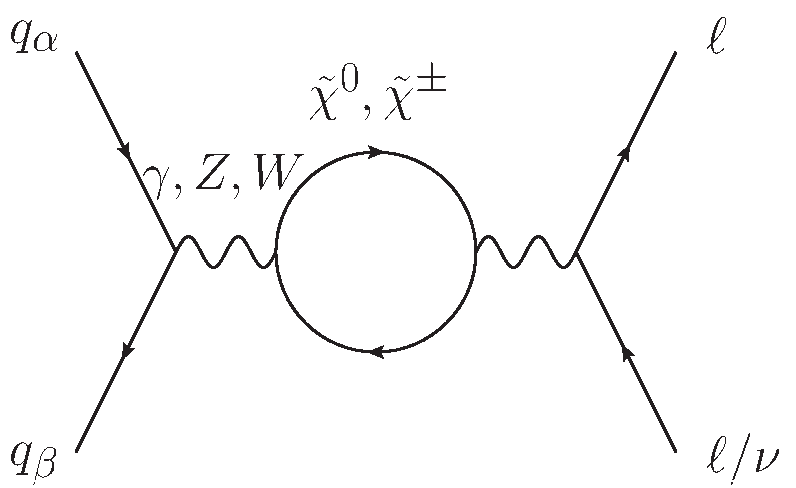
\includegraphics[width=0.5\hsize]{NC_CC_WIMP.pdf}
  \caption{WIMP effect on the Drell-Yan processes considered in this section.}
  \label{fig:NC_CC_WIMP}
\end{figure}

So far, we have discussed several ways to search for WIMPs using DM searches and collider experiments.
We have seen that, while WIMPs with relatively large $SU(2)_L$ charges such as Wino and the 5-plet fermion are promising for these searches, Higgsino is typically more challenging to probe.
Given this situation, another search strategy attracts a lot of attention~\cite{Chigusa:2018vxz, Abe:2019egv, Alves:2014cda, Harigaya:2015yaa, Gross:2016ioi, Farina:2016rws, Matsumoto:2017vfu, DiLuzio:2018jwd, Matsumoto:2018ioi} that probes WIMPs via the electroweak precision measurement at colliders.
It utilizes a pair production of charged leptons or that of a charged lepton and a neutrino, where WIMPs affect the pair production processes through the vacuum polarization of the electroweak gauge bosons as shown in Fig.~\ref{fig:NC_CC_WIMP}.
It is an indirect search method in the sense that it does not produce on-shell WIMPs as final states.

There are several virtues in this method such as the robustness against the change of the lifetime and the decay modes of WIMPs and the characteristic dip-like shape of the invariant mass distributions at the value close to twice the WIMP mass as we will see below.
We will see that the latter point helps us to distinguish the WIMP effects from backgrounds and systematic errors.
However, the obtained reach for Higgsino in most of the literature is still unsatisfactory since the use of the LHC or lepton colliders gives us only a small number of events at the position of the dip for a heavy Higgsino, which results in the reach much below the thermal Higgsino DM mass $m_\chi \sim 1\,\mathrm{TeV}$.

\begin{figure}[t]
  \centering
  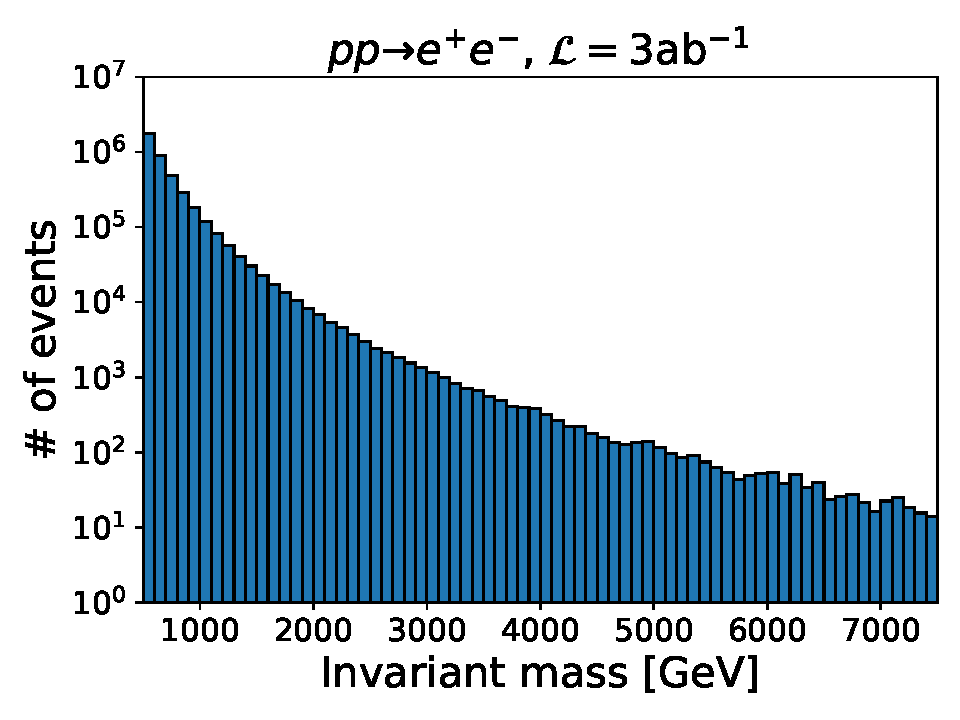
\includegraphics[width=0.5\hsize]{histMee.pdf}
  \caption{
    Invariant mass distribution of the pair-produced electrons at a $100\,\mathrm{TeV}$ collider with the integrated luminosity $\mathcal{L} = 3\,\mathrm{ab}^{-1}$.
  }
  \label{fig:histMee}
\end{figure}

Thus, in this section, we pursue this indirect search method further, considering a much higher CM energy using the future $100\,{\rm TeV}$ hadron colliders such as FCC-hh~\cite{Mangano:2016jyj, Contino:2016spe, Golling:2016gvc, Benedikt:2651300} and SppC~\cite{CEPC-SPPCStudyGroup:2015csa, CEPC-SPPCStudyGroup:2015esa}.
We concentrate on the Drell-Yan processes that have two charged leptons or mono-lepton plus a neutrino in the final state since they provide a very clean signal without any hadronic jets at least from the final state particles.
In Fig.~\ref{fig:histMee}, we show the invariant mass distribution of the pair produced electrons, for example, at a $100\,\mathrm{TeV}$ collider with the integrated luminosity $\mathcal{L} = 3\,\mathrm{ab}^{-1}$.
As we will discuss in Sec.~\ref{sec_event} in more detail, the NLO QCD effect is taken into account and \texttt{NNPDF2.3QED} with $\alpha_s (M_Z) = 0.118$~\cite{Ball:2013hta} is used as a canonical set of PDFs.
In the figure, events are divided into bins with equal width of $100\,\mathrm{GeV}$.
Thanks to the large CM energy, there are roughly $10^4$ events around the invariant mass of $2\,\mathrm{TeV}$ that can be used to probe the $\mathcal{O}(1)\,\%$ effect of the new physics, which will be turned out to be useful for the $1\,\mathrm{TeV}$ Higgsino search.

Below, we will show that the indirect search method provides \textit{a comparable or better experimental reach for Higgsino} compared to the direct production search of WIMPs at future colliders~\cite{Low:2014cba, Cirelli:2014dsa, Han:2018wus, Mahbubani:2017gjh}.
Besides, we demonstrate for the first time that the indirect search method can be applied not only to discover WIMPs but also \textit{to investigate their properties, such as charges, masses, and spins.}
To this end, it is important to consider both the charged current (CC) process with two-lepton final state and the neutral current (NC) process with mono-lepton final state to break some degeneracy among different WIMP charge assignments; the NC and CC processes depend on different combinations of the $SU(2)_L$ and $U(1)_Y$ charges of WIMP, and hence the inclusion of both processes allows us to extract these charges separately.

This section is based on our works \cite{Chigusa:2018vxz, Abe:2019egv}.


%%%%%%%%%%%%%%%%%%%%%%%%%%%%%%%%%%%%%%%%%%%%%%%%%%
\subsection{WIMP effect on the Drell-Yan processes}
\label{sec:WIMP}
%%%%%%%%%%%%%%%%%%%%%%%%%%%%%%%%%%%%%%%%%%%%%%%%%%

We investigate contributions of the WIMPs to the Drell-Yan processes through the vacuum polarization of the electroweak gauge bosons at the loop level.
Throughout this section, we assume that all the other beyond the SM particles are heavy enough so that they do not affect the following discussion.
After integrating out the WIMPs, the effective lagrangian relevant for our analysis is expressed as
\begin{align}
 \mathcal{L}_{\rm eff} = \mathcal{L}_{\rm SM} + C_2 g^2\, W_{\mu \nu}^a
 f\left(-\frac{D^2}{m^2}\right) W^{a\mu\nu} + C_1 g'^2\, B_{\mu\nu}
 f\left(-\frac{\partial^2}{m^2}\right) B^{\mu\nu},\label{eq_lag}
\end{align}
where $\mathcal{L}_{\rm SM}$ is the SM Lagrangian, $D$ is a covariant derivative, $m$ is the WIMP mass,\footnote
{
  Here we neglect a small mass splitting among the $SU(2)_L$ multiplet.
}
$g$ and $g'$ are the $SU(2)_L$ and $U(1)_Y$ gauge coupling constants, and $W_{\mu\nu}^a$ and $B_{\mu\nu}$ are the field strength associated with the $SU(2)_L$ and $U(1)_Y$ gauge group, respectively.
The function $f(x)$ is defined as \cite{Matsumoto:2017vfu}
\begin{align}
  f(x) = \begin{cases}
    \displaystyle{\frac{1}{16\pi^2} \int_0^1 dy\, (1-2y)^2 \ln (1-
    y(1-y)x - i0)} & {\rm (Scalar)},\\[5mm]
	  %%
    \displaystyle{\frac{1}{16\pi^2} \int_0^1 dy\, y(1-y) \ln (1 -
	  y(1-y)x - i0)} & {\rm (Fermion)},
  \end{cases}\label{eq_f}
\end{align}
where the first (second) line corresponds to a scalar (fermionic) WIMP, respectively.\footnote
{
  If a WIMP interacts only through the electroweak interaction, its decay width is of $\mathrm{O}(1)\%$ or less of its mass even if it is unstable.
  We assume that this is the case, and neglect the small effect on the function $f(x)$ due to the small decay width.
  Also, $f(x)$ corresponds to the finite part of the WIMP loop contribution after performing the renormalization in the $\overline{\mathrm{MS}}$ scheme.
}
The coefficients $C_1$ and $C_2$ for an $SU(2)_L$ $n$-plet WIMP with hypercharge $Y$ are given by
\begin{align}
 C_1 &= \frac{\kappa}{8} n Y^2,\label{eq_C1}\\
 %%
 C_2 &= \frac{\kappa}{8} I(n),\label{eq_C2}
\end{align}
where $\kappa = 1, 2, 8, 16$ for a real scalar, a complex scalar, a Weyl or Majorana fermion, and a Dirac fermion, respectively.
$I(n)$ is the Dynkin index for the $n$ dimensional representation of $SU(2)_L$ defined in Eq.~\eqref{eq:Dynkin}.
The coefficients are uniquely determined by the representation of the WIMPs.
For example, $(C_1, C_2) = (1, 1)$ for Higgsino, and $(C_1, C_2) = (0, 2)$ for Wino.
We emphasize that, contrary to the usual effective field theory, our prescription is equally applied when the typical scale of the gauge boson four-momentum $q$ is larger than the WIMP mass scale $m$ since we do not perform a derivative expansion of $f$ in
Eq.~\eqref{eq_lag}.
It is important because, as we see soon, the effect of the WIMPs is maximized when $q^2\sim m^2$, where the derivative expansion is not applicable.

\begin{table}[t]
  \centering
  \def\arraystretch{1.2}
  \begin{tabular}{c|cccccc}
    Fermion $f$ & $v_f^{(\gamma)}$ & $a_f^{(\gamma)}$ & $v_f^{(Z)}$ & $a_f^{(Z)}$ & $v_f^{(W)}$ & $a_f^{(W)}$ \\ \hline
    up-type quark & $\frac{2}{3}e$ & 0 & $(\frac{1}{4}-\frac{2}{3}s_W^2) g_Z$ & $-\frac{1}{4}g_Z$ & $\frac{1}{2\sqrt{2}}g$ & $-\frac{1}{2\sqrt{2}}g$ \\
    down-type quark & $-\frac{1}{3}e$ & 0 & $(-\frac{1}{4}+\frac{1}{3}s_W^2)g_Z$ & $\frac{1}{4}g_Z$ & $\frac{1}{2\sqrt{2}}g$ & $-\frac{1}{2\sqrt{2}}g$ \\
    lepton & $-e$ & 0 & $(-\frac{1}{4}+s_W^2)g_Z$ & $\frac{1}{4}g_Z$ & $\frac{1}{2\sqrt{2}}g$ & $-\frac{1}{2\sqrt{2}}g$ \\
  \end{tabular}
  \caption{Coefficients of the weak interaction defined as
    $\Gamma_f^{(V)} \equiv v_f^{(V)} + a_f^{(V)} \gamma_5$.  Here, $e = g
    s_W$ and $g_Z = g / c_W$, where $s_W \equiv \sin \theta_W$ and $c_W
    \equiv \cos \theta_W$ with $\theta_W$ being the weak mixing angle.}
  \label{table_weak}
\end{table}

At the leading order (LO), we are interested in $u(p)~\bar{u}(p') \to \ell^{-}(k)~\ell^{+}(k')$ and $d(p)~\bar{d}(p') \to \ell^{-}(k)~\ell^{+}(k')$ as the NC processes and $u(p)~\bar{d}(p') \to \nu(k)~\ell^{+}(k')$ and $d(p)~\bar{u}(p') \to \ell^{-}(k)~\bar{\nu}(k')$ as the CC processes.
Here, $u$ and $d$ collectively denote up-type and down-type quarks, respectively, and $p, p', k$, and $k'$ are initial and final state momenta.
In the SM, the amplitudes for both the NC and CC processes at the LO are expressed as
\begin{align}
 \mathcal{M}_{\rm SM} = \sum_{V} \frac{\left[ \bar{v}(p')
 \gamma^\mu \Gamma_q^{(V)} u(p) \right] \left[ \bar{u}(k) \gamma_\mu
 \Gamma_{\ell}^{(V)} v(k') \right]}{s' - m_V^2},\label{eq_m_sm}
\end{align}
where $\sqrt{s'}$ is the invariant mass of the final state leptons, which is denoted as $m_{\ell\ell}$ for the NC processes and $m_{\ell\nu}$ for the CC processes.
The relevant gauge bosons are $V = \gamma, Z$ for the NC processes and $V = W^\pm$ for the CC processes, with $m_V$ being the corresponding gauge boson mass.
In addition,
\begin{align}
  \Gamma_f^{(V)} \equiv v_f^{(V)} + a_f^{(V)} \gamma_5,
\end{align}
with $v_f^{(V)}$ and $a_f^{(V)}$ given in Tab.~\ref{table_weak}.
The WIMP contribution is given by
\begin{align}
 \mathcal{M}_{\rm WIMP} = \sum_{V,V'} C_{VV'} s' f\left(\frac{s'}{m^2}\right)
 \frac{\left[ \bar{v}(p') \gamma^\mu \Gamma_q^{(V)} u(p) \right]
 \left[ \bar{u}(k) \gamma_\mu \Gamma_\ell^{(V')} v(k') \right]}
 {(s'-m_V^2)(s'-m_{V'}^2)},\label{eq_m_WIMP}
\end{align}
where $C_{\gamma \gamma} = 4(C_1 g'^2 c_W^2 + C_2 g^2 s_W^2)$, $C_{\gamma Z} = C_{Z \gamma} = 4(C_2 g^2 - C_1 g'^2) s_W c_W$, $C_{Z Z} = 4(C_1 g'^2 s_W^2 + C_2 g^2 c_W^2)$, and $C_{WW} = 4 C_2 g^2$.
Again $V, V' = \gamma, Z$ for the NC processes and $V, V' = W^\pm$ for the CC processes.

We use $d\Pi_{\mathrm{LIPS}}$ for a Lorentz invariant phase space factor for the two-particle final state.
Then, using Eqs.~\eqref{eq_m_sm} and~\eqref{eq_m_WIMP}, we define
\begin{align}
 \frac{d \sigma_{\rm SM}}{d\sqrt{s'}} &= \sum_{\alpha, \beta}
 \frac{dL_{\alpha \beta}}{d\sqrt{s'}} \int d\Pi_{\mathrm{LIPS}}\, \left| \mathcal{M}_{\rm SM} \left( q_\alpha q_\beta \to \ell\ell / \ell\nu \right) \right|^2,\label{eq_sig_sm}\\
 %%
 \frac{d \sigma_{\rm WIMP}}{d\sqrt{s'}} &= \sum_{\alpha, \beta}
 \frac{dL_{\alpha \beta}}{d\sqrt{s'}} \int d\Pi_{\mathrm{LIPS}}\, 2 \Re \left[ \mathcal{M}_{\rm SM}
 \mathcal{M}_{\rm WIMP}^{*} \left( q_\alpha q_\beta \to \ell\ell / \ell\nu
 \right) \right],\label{eq_sig_WIMP}
\end{align}
where we take the average and summation over spins.\footnote{
  In Eq.~\eqref{eq_sig_WIMP}, we only take into account the contribution from WIMPs at the leading order of $g^{'2}$ and $g^2$, which corresponds to the real part of the loop function Eq.~\eqref{eq_f}.
  The contribution from the imaginary part may be enhanced by a sizable numerical factor, but we neglect it simply because it is a higher order term of the gauge coupling expansion.
}
Here, $dL_{\alpha \beta} / d\sqrt{s'}$ is the so-called luminosity function for a fixed
$\sqrt{s'}$:
\begin{align}
 \frac{d L_{\alpha \beta}}{d\sqrt{s'}} \equiv \frac{1}{s} \int_0^1 dx_1
 dx_2~f_\alpha(x_1) f_\beta(x_2) \delta\left(\frac{s'}{s} - x_1 x_2\right),
\end{align}
where $\alpha$ and $\beta$ denote species of initial partons, $\sqrt{s} = 100\,{\rm TeV}$, and $f_a(x)$ is the PDF used in Sec.~\ref{sec:wimp_production}.
Eq.\,\eqref{eq_sig_sm} represents the SM cross section, while Eq.\,\eqref{eq_sig_WIMP} the WIMP contribution to the cross section.
For the statistical treatment in the next section, we introduce a parameter $\mu$ that parametrizes the strength of the WIMP effect and express the cross section with $\mu$ as
\begin{align}
 \frac{d\tilde{\sigma}}{d\sqrt{s'}} =
 \frac{d\sigma_{\rm SM}}{d\sqrt{s'}}
 + \mu \frac{d\sigma_{\rm WIMP}}{d\sqrt{s'}}.
 \label{eq_diffcrosssection}
\end{align}
Obviously, $\mu=0$ corresponds to the pure SM, while $\mu=1$ corresponds to the SM$+$WIMP model.
Hereafter, we use
\begin{align}
 \delta_\sigma ( \sqrt{s'} ) \equiv \frac{d\sigma_{\rm
 WIMP} / d\sqrt{s'}}{d\sigma_{\rm SM} /
 d\sqrt{s'}},\label{eq_dsigma}
\end{align}
to denote the correction from the WIMP.
Note that this ratio remains unchanged even if we take into account the next-to-leading order (NLO) QCD effect because the EWIMPs affect the cross sections only through the vacuum polarization.\footnote
{
  When the NLO QCD effect is included, one of the initial partons can be gluon with the real emission of one jet in the final state.
  However, we can easily see that $\delta_\sigma^{ug}$ = $\delta_\sigma^{uu}$ and so on.
}

\begin{figure}[t]
  \centering
  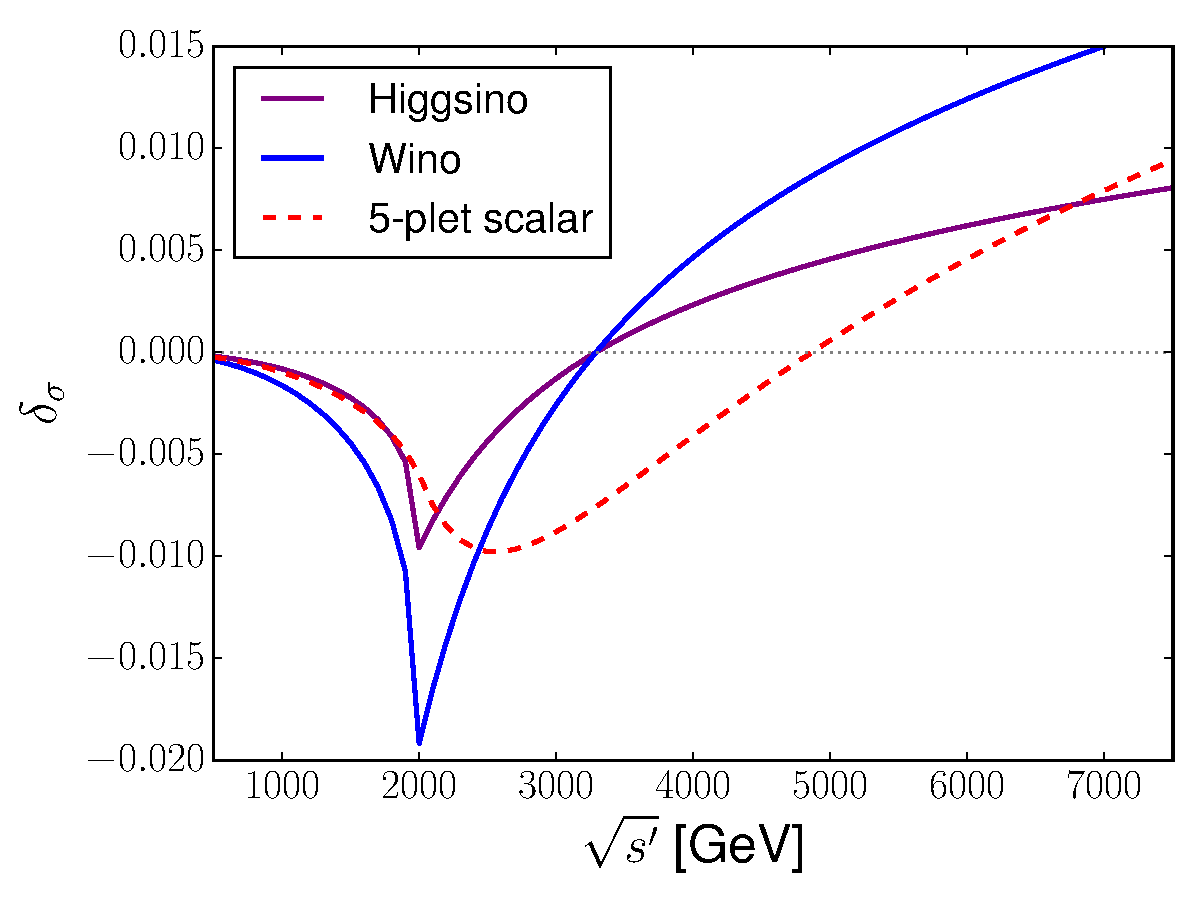
\includegraphics[width=0.5\hsize]{sqsp_vs_del.pdf}
  \caption{
    $\delta_\sigma$ for the CC processes as a function of $\sqrt{s'} = m_{\ell\nu}$.
    The purple, blue, and red lines correspond to Higgsino, Wino, and 5-plet real scalar, respectively.
  }
  \label{fig_sqsp_vs_del}
\end{figure}

In Fig.~\ref{fig_sqsp_vs_del}, we plot $\delta_\sigma$ for the CC processes as a function of $\sqrt{s'}$.
The purple, blue, and red lines correspond to Higgsino, Wino, and 5-plet scalar, respectively.
There is a dip around $\sqrt{s'} = 2m$ for all the cases of the WIMPs which originates from the loop function $f$ in Eq.~\eqref{eq_f}.
The WIMP contributions to the NC processes show a similar dip structure that again comes from $f$.
This dip is crucial not only for the discovery of the WIMP signal (see Sec.~\ref{sec_detection}) but also for the determination of the properties of the WIMPs (see Sec.~\ref{sec_property}).
In particular, the WIMP mass can be extracted from the dip position, while the WIMP charges ($n$ and $Y$) can be determined from the depth of the dip.
The negative sign of the WIMP contributions can be understood from the consideration using the optical theorem and the analytic structure of the loop function.
See Appendix \ref{sec:reim} for the detailed discussion.

\begin{figure}[t]
  \centering
  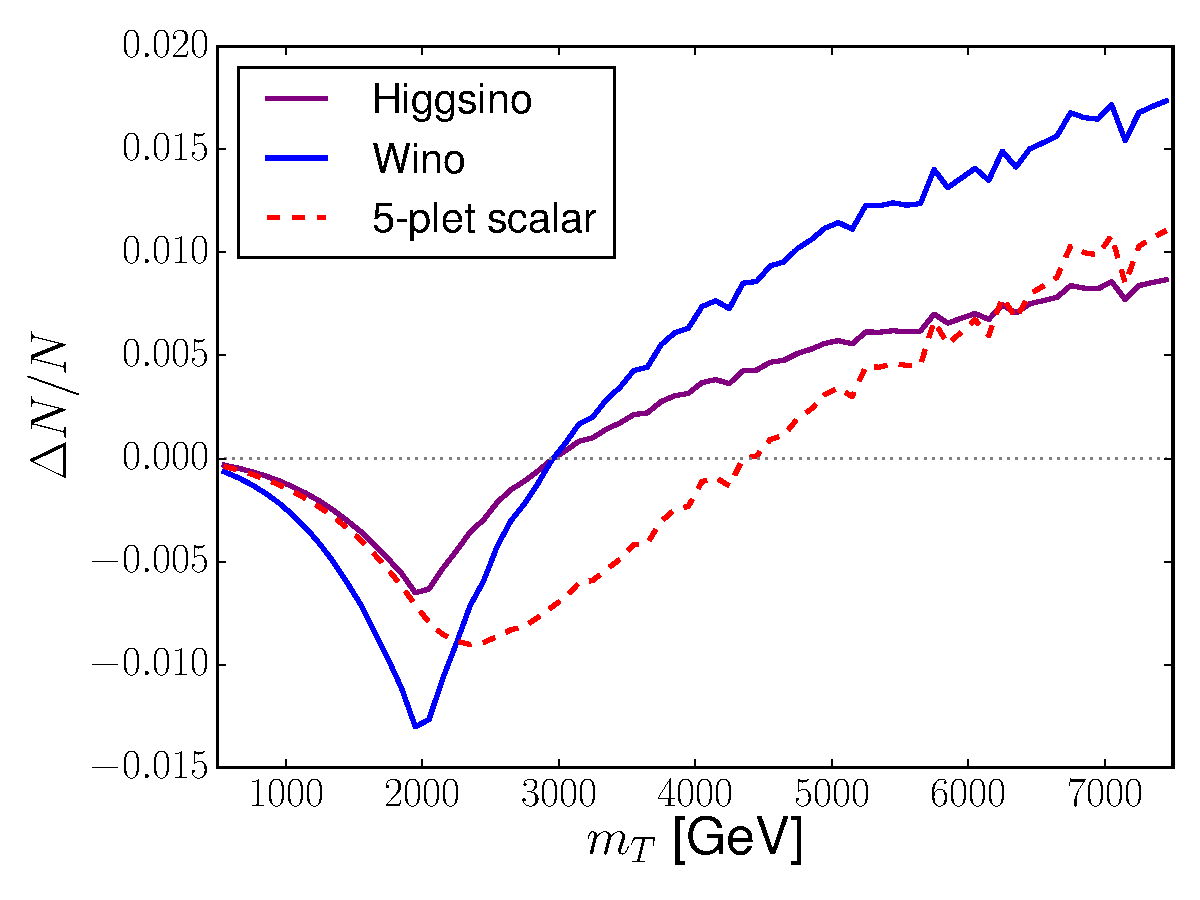
\includegraphics[width=0.5\hsize]{mT_vs_del.pdf}
  \caption{
    The WIMP effect on the ratio of the number of events $\Delta N / N$ as a function of $m_T$.
    The line colors are the same as Fig.~\ref{fig_sqsp_vs_del}.
  }
  \label{fig_mT_vs_dN}
\end{figure}

For the NC processes, the momenta of two final state charged leptons are measurable and we can use the invariant mass distribution of the number of events for the study of the WIMPs.
For the CC processes, on the contrary, we cannot measure the momentum of the neutrino in real experiments, and hence we instead use the missing transverse momentum $\Slash{p}_T$.
We use the transverse mass defined as
\begin{align}
  m_T^2 \equiv 2 p_{T, \ell}\,\Slash{p}_T \left( 1-\cos \phi \right),
\end{align}
where $p_{T, \ell}$ denotes the transverse momentum of the charged lepton and $\phi$ is the difference between the azimuth angles of $p_{T,\ell}$ and $\Slash{p}_T$.
The important property of $m_T$ is that the distribution of $m_T$ peaks at $m_T = m_{\ell\nu}$ (see Appendix~\ref{sec:mT} for more detailed description of the quantity $m_T$).
Because of this property, the characteristic shape of $\delta_\sigma$ remains in the $m_T$ distribution in the CC events.
To see this, we plot in Fig.~\ref{fig_mT_vs_dN} the WIMP effect on the number of events as a function of $m_T$.
Here, the vertical axis is the ratio of the WIMP correction to the number of events $\Delta N$ to the number of events in the SM $N$ for each bin with the bin width of $100\, {\rm GeV}$.\footnote
{
  Just for an illustrative purpose, we generate events corresponding to the integrated luminosity $\mathcal{L} = 1\,\mathrm{ab}^{-1}$ for this figure, which is not the same luminosity as we use in the next section (see Sec.~\ref{sec_event} for details of the event generation).
}
We find that the dip structure remains in the $m_T$ distribution, though the depth of the dip is smaller compared to the $m_{\ell\nu}$ distribution.


%%%%%%%%%%%%%%%%%%%%%%%%%%%%%%%%%%%%%%%%%%%%%%%%%%
\subsection{Analysis}
\label{sec:analysis}
%%%%%%%%%%%%%%%%%%%%%%%%%%%%%%%%%%%%%%%%%%%%%%%%%%


%%%%%%%%%%%%%%%%%%%%%%%%%%%%%%%%%%%%%%%%%%%%%%%%%%
\subsubsection{Event generation}
\label{sec_event}
%%%%%%%%%%%%%%%%%%%%%%%%%%%%%%%%%%%%%%%%%%%%%%%%%%

Now we discuss how well we can extract information about WIMPs from the invariant mass and transverse mass distributions for the processes of our concern at future $100\,\mathrm{TeV}$ $pp$ collider experiments.
We take into account the effects of the next-to-leading order QCD corrections in the events as well as detector effects through Monte-Carlo simulations.

In our analysis, we first generate the SM event sets for the NC processes $pp\to e^{-}e^{+} / \mu^{-}\mu^{+}$ and the CC processes $pp\to e^{\pm}\nu_e / \mu^{\pm}\nu_\mu$.
We use \texttt{MadGraph5\_aMC@NLO} (\texttt{v2.6.3.2})~\cite{Alwall:2011uj, Alwall:2014hca} for the event generation with the successive use of \texttt{Pythia8}~\cite{Sjostrand:2014zea} for the parton shower and the hadronization and \texttt{Delphes} (\texttt{v3.4.1})~\cite{deFavereau:2013fsa} with the card {\tt FCChh.tcl} for the detector simulation.
We use \texttt{NNPDF2.3QED} with $\alpha_s (M_Z) = 0.118$~\cite{Ball:2013hta} as a canonical set of PDFs.
For the renormalization and factorization scales, we use the default values of \texttt{MadGraph5\_aMC@NLO}, i.e., the central $m_T^2$ scale after $k_T$-clustering of the event (which we denote by $Q$).
We take into account the NLO QCD effect by the \verb|[QCD]| option of \verb|MadGraph5_aMC@NLO| which enhances the cross section roughly by a factor of $2$ compared to the LO calculation.\footnote
{
  This large enhancement implies that the next-to-next-to-leading order QCD effect may also have a non-negligible effect on the cross section, and its calculation remains as a future task.
  However, due to its smooth dependence on $\sqrt{s'}$, it may not much affect the detection reach of the EWIMPs.
  See Sec.~\ref{sec_statistical} for the details.
}
The events are binned by the characteristic mass $m_{\mathrm{char}}$ for each process: we use the lepton invariant mass $m_{\mathrm{char}} = m_{\ell\ell}$ for the NC processes, and the transverse mass $m_{\mathrm{char}} = m_T$ for the CC processes, respectively.
In both cases, we generated events with the characteristic mass within the range of $500\,\mathrm{GeV} < m_\mathrm{char} < 7.5\,\mathrm{TeV}$ and divide them into $70$ bins with an equal width of $100\,\mathrm{GeV}$.

As for the event selection by a trigger, we may have to impose some cut on the lepton transverse momentum $p_T$.
As we will see, we concentrate on events with high $p_T$ charged lepton(s) with which we expect the event may be triggered.
For the NC processes, we use events with at least two high $p_T$ leptons.  For our analysis, we use events with $m_{\ell\ell}>500\ {\rm GeV}$; we assume that such events are triggered by using two energetic charged leptons so that we do not impose any other kinematical requirement at the parton level.\footnote{
  Note that the simplified geometry of detector layout is included in the \texttt{Delphes} card and, for example, muons with large absolute pseudorapidity $|\eta| > 6$ are automatically neglected at the detector simulation.
}
On the contrary, the CC events are characterized only by a lepton and a missing transverse momentum.
For such events, we require that the $p_T$ of the charged lepton should be larger than $500\,\mathrm{GeV}$.
\footnote{
  In the ATLAS analysis of the mono-lepton signal during the 2015 (2016) data taking period~\cite{Aaboud:2017efa}, they use the event selection condition $p_T > 24\, (60)\,\mathrm{GeV}$ for leptons that satisfy the \textit{medium} identification criteria.
  In the CMS analysis during the period on 2016~\cite{Sirunyan:2018mpc}, they use the condition $p_T > 130 (53)\, \mathrm{GeV}$ for an electron (a muon).
}
For the CC events, the cut reduces the number of events in particular for the bins with the low transverse mass $m_T \sim 500\, \mathrm{GeV}$, and thus affects the sensitivity of the CC processes to relatively light WIMPs.
We will come back to this point later.


The WIMP effect is incorporated by rescaling the SM event by $\delta_\sigma$ defined in Eq.~\eqref{eq_dsigma}.
With the parameter $\mu$ defined in Eq.~\eqref{eq_diffcrosssection}, the number of events corresponding to the SM+WIMP hypothesis in $i$-th bin, characterized by $m_{i, \mathrm{min}} < m_{\mathrm{char}} < m_{i, \mathrm{max}}$, is
\begin{align}
  x_{f,i} (\mu) = \sum_{\substack{\text{events that satisfy}\\m_{i, \mathrm{min}} < m_{\mathrm{char}} < m_{i, \mathrm{max}}}}
  \left[
    1 + \mu \delta_\sigma (\sqrt{s'})
  \right],
  \label{eq_n_tot}
\end{align}
where the sum runs over all the events of the final state $f$ whose characteristic mass $m_{\mathrm{char}}$ (after taking into account the detector effects) falls into the bin.
Note that the true value of $\sqrt{s'}$ should be used for each event for the computation of $\delta_\sigma$: we extract it from the hard process information.\footnote
{
	The $p_T$ cut for the CC process does not affect this estimation since the WIMP does not modify the angular distribution of the final lepton and neutrino for the CC process.
}


%%%%%%%%%%%%%%%%%%%%%%%%%%%%%%%%%%%%%%%%%%%%%%%%%%
\subsubsection{Statistical treatment}
\label{sec_statistical}
%%%%%%%%%%%%%%%%%%%%%%%%%%%%%%%%%%%%%%%%%%%%%%%%%%

We now explain the statistical method we will adopt in our analysis.
Throughout this section, we rely on the so-called profile likelihood method, which is described in detail in Appendix \ref{sec:profile}.
We collectively denote our theoretical model as $\bm{x}_f(\mu) = \{ x_{f,i} (\mu) \}$, where $x_{f,i}(\mu)$ is given by Eq.~\eqref{eq_n_tot}.
We denote the experimental data set as $\check{\bm{x}}_f$ that in principle is completely unrelated to our theoretical model $\bm{x}_f(\mu)$.
Since we do not have an actual experimental data set for $100~\,\mathrm{TeV}$ colliders for now, however, we take $\check{\bm{x}}_f = \bm{x}_f(\mu = 1)$ (for some fixed values of the WIMP mass and charges) throughout our analysis, assuming that the WIMP does exist.  In particular, this choice tests the SM-only hypothesis if we take our theoretical model as $\bm{x}_f(\mu=0)$.

If the expectation values of $x_{f,i} (\mu)$ are precisely known, the sensitivity to WIMPs can be studied only with statistical errors.
In reality, however, the computation of $x_{f,i} (\mu)$ suffers from various sources of uncertainties, which results in systematic errors in our theoretical model.
The sources include errors in the integrated luminosity, the beam energy, choices of the renormalization and the factorization scales, choices of PDF, the pile-up effect, higher order corrections to the cross section, and so on.
In order to deal with these uncertainties, we introduce sets of free parameters $\bm{\theta}_f = \{ \theta_{f,\alpha} \}$ (i.e. nuisance parameters) which absorb (smooth) uncertainties of the number of events, and modify our theoretical model as
\begin{align}
  \tilde{x}_{f,i} (\bm{\theta}_f, \mu) \equiv x_{f,i} (\mu)
  f_{\mathrm{sys}, i}(\bm{\theta}_f),\label{eq_xtilde}
\end{align}
where $f_{\mathrm{sys}, i}(\bm{\theta}_f)$ is a function that satisfies $f_{\mathrm{sys}, i}(\bm{0}) =1$.
We expect that, if the function $f_{\mathrm{sys}, i}$ is properly chosen, the true distribution of the number of events in the SM is given by $\tilde{\bm{x}}_f (\bm{\theta}_f,0) = \{ \tilde{x}_{f,i} (0) f_{\mathrm{sys}, i}(\bm{\theta}_f)\}$ for some value of $\bm{\theta}_f$.
In our analysis, we adopt the five parameters fitting function given by~\cite{Aaltonen:2008dn}
\begin{align}
  f_{\mathrm{sys}, i} (\bm{\theta}_f) =
  e^{\theta_{f,1}} (1 - p_i)^{\theta_{f,2}}
  p_i^{(\theta_{f,3} + \theta_{f,4} \ln p_i + \theta_{f,5} \ln^2 p_i)},
  \label{eq_f_theta}
\end{align}
where $p_i = 2m_{i} / \sqrt{s}$ with $m_i$ being the central value of the lepton invariant mass (transverse mass) of the $i$-th bin for the NC (CC) processes.
As we will see, the major effects of systematic errors can be absorbed into $\bm{\theta}_f$ with this fitting function.

To test the SM-only hypothesis, we define the following test statistic~\cite{Cowan:2010js}:
\begin{align}
  q_0 \equiv -2 \sum_{f=\ell \ell, \ell \nu} \ln \frac
  {L(\check{\bm{x}}_f ; \doublehat{\bm{\theta}}_f, \mu=0)}
  {L(\check{\bm{x}}_f ; \hat{\bm{\theta}}_f, \hat{\mu})}.
  \label{eq_q0}
\end{align}
Here, $\doublehat{\bm{\theta}}_f$ and $\{ \hat{\bm{\theta}}_f, \hat{\mu} \}$ are determined so that $\prod_f L(\check{\bm{x}}_f ; \bm{\theta}_f, \mu=0)$ and $\prod_f L(\check{\bm{x}}_f ; \bm{\theta}_f, \mu)$ are maximized, respectively.
The likelihood function is defined as
\begin{align}
  L(\check{\bm{x}}_f ; \bm{\theta}_f, \mu) &\equiv
  L_{\bm{\theta}_f} (\check{\bm{x}}_f ; \mu) L'(\bm{\theta}_f ; \bm{\sigma}_f),
  \label{eq_L}
\end{align}
where
\begin{align}
  L_{\bm{\theta}_f} (\check{\bm{x}}_f ; \mu) &\equiv
  \prod_{i} \exp \left[
  -\frac{(\check{x}_{f,i} - \tilde{x}_{f,i} (\bm{\theta}_f, \mu))^2}
  {2 \tilde{x}_{f,i} (\bm{\theta}_f, \mu)}
  \right],
  \label{eq_Ltheta}\\
  %%
  L'(\bm{\theta}_f ; \bm{\sigma}_f) &\equiv
  \prod_{\alpha} \exp \left[
  - \frac{\theta_{f,\alpha}^2}{2\sigma_{f,\alpha}^2}
  \right].
  \label{eq_Lprime}
\end{align}
The product in Eq.\,\eqref{eq_Ltheta} runs over all the bins, while the product in Eq.\,\eqref{eq_Lprime} runs over all the free parameters we introduced.
For each $\theta_{f, \alpha}$, we define the ``standard deviation'' $\sigma_{f, \alpha}$, which parametrizes the possible size of $\theta_{f, \alpha}$ within the SM with the
systematic errors.\footnote
{
  Here we assume the Gaussian form for the nuisance parameter distribution.  The dependence of the results on the choice of the distribution will be discussed later in Sec.~\ref{sec_detection}.
}
If the systematic errors are negligible compared with the statistical error, we can take $\bm{\sigma}_f \to \bm{0}$, while the analysis with $\bm{\sigma}_f \to \infty$ assumes no knowledge of systematic errors and gives a conservative result.
We identify $\sqrt{q_0} = 5$ $(1.96)$ as the detection reach at the $5\sigma$ ($95\,\%$ C.L.) level, since $q_0$ asymptotically obeys a chi-square distribution with the degree of freedom one.

In order to determine $\bm{\sigma}_f$, we consider the following sources of the systematic errors:
\begin{itemize}
  \item Luminosity ($\pm 5\,\%$ uncertainty is assumed),
  \item Renormalization scale ($2Q$ and $Q/2$, instead of $Q$),
  \item Factorization scale ($2Q$ and $Q/2$, instead of $Q$),
  \item PDF choice (We use $101$ variants of \texttt{NNPDF2.3QED} with $\alpha_s (M_Z) = 0.118$~\cite{Ball:2013hta} provided by \texttt{LHAPDF6}~\cite{Buckley:2014ana} with IDs ranging from $244600$ to $244700$).
\end{itemize}
The values of $\bm{\sigma}_f$ are determined as follows.
Let $\bm{y}_f$ be the set of number of events in the SM for the final state $f$ with the canonical choices of the parameters, and $\bm{y}'_f$ be that with one of the sources of the systematic errors being varied.
We minimize the chi-square function defined as
\begin{align}
  \chi^2_f &\equiv \sum_i \frac
  {\left( y_{f,i}' - \tilde{y}_{f,i} (\bm{\theta}_f) \right)^2}
  {\tilde{y}_{f,i} (\bm{\theta}_f)},
\end{align}
where
\begin{align}
  \tilde{y}_{f,i} (\bm{\theta}_f) &\equiv
  y_{f,i} f_{\mathrm{sys},i} (\bm{\theta}_f),
\end{align}
for each final state $f$, and determine the best-fit values of $\bm{\theta}_f$ for each set of $\bm{y}'_f$.
We repeat this process for different sets of $\bm{y}'_f$, and $\bm{\sigma}_f$ are determined from the distributions of the best-fit values of $\bm{\theta}_f$.
For example, let us denote the best-fit values for the fit associated with the luminosity errors $\pm 5\%$ as $\bm{\theta}_f^{\pm}$.
We estimate $\bm{\sigma}_f$ associated with these errors, denoted here as $\bm{\sigma}_f^{\mathrm{lumi.}}$, as
\begin{align}
  \sigma_{f,\alpha}^{\mathrm{lumi.}} = \sqrt{\frac{(\theta_{f,\alpha}^{+})^2 + (\theta_{f,\alpha}^{-})^2}{N}},
\end{align}
where $N$ denotes the number of fitting procedures we have performed: $N=2$ for this case.
We estimate $\bm{\sigma}_f$ associated with the other sources of the errors, denoted as $\bm{\sigma}_f^{\mathrm{ren.}}$, $\bm{\sigma}_f^{\mathrm{fac.}}$, and $\bm{\sigma}_f^{\mathrm{PDF}}$, in a similar manner.
Finally, the total values of $\bm{\sigma}_f$ are obtained by combining all the sources together as\footnote
{
  There may be some correlations between the distribution of nuisance parameters $\bm{\theta}_{f}$.
  After the $100\,\mathrm{TeV}$ collider experiments will start and the sufficient amount of data will be accumulated, we should extract the information of correlations and use it to perform the analysis.
  However, because the real data does not exist yet, we rely on a simplified analysis in this section, treating each of them as obeying to an independent Gaussian distribution.
}
\begin{align}
  \sigma_{f,\alpha} = \sqrt{(\sigma_{f,\alpha}^{\mathrm{lumi.}})^2
  + (\sigma_{f,\alpha}^{\mathrm{ren.}})^2
  + (\sigma_{f,\alpha}^{\mathrm{fac.}})^2
  + (\sigma_{f,\alpha}^{\mathrm{PDF}})^2}.
  \label{eq_comb_sig}
\end{align}

\begin{table}[t]
  \centering
  \begin{tabular}{c|ccccc}
    Sources of systematic errors & $\sigma_{ee,1}$ & $\sigma_{ee,2}$ & $\sigma_{ee,3}$ & $\sigma_{ee,4}$ & $\sigma_{ee,5}$ \\ \hline
    Luminosity: $\pm 5\,\%$ ($\bm{\sigma}_{ee}^{\mathrm{lumi.}}$) & $0.05$ & $0$ & $0$ & $0$ & $0$ \\
    Renormalization scale: $2Q, Q/2$ ($\bm{\sigma}_{ee}^{\mathrm{ren.}}$) & $0.4$ & $0.6$ & $0.3$ & $0.05$ & $0.004$ \\
    Factorization scale: $2Q, Q/2$ ($\bm{\sigma}_{ee}^{\mathrm{fac.}}$) & $0.3$ & $0.5$ & $0.2$ & $0.06$ & $0.004$ \\
    PDF choice ($\bm{\sigma}_{ee}^{\mathrm{PDF}}$) & $0.4$ & $0.7$ & $0.3$ & $0.06$ & $0.004$
  \end{tabular}
  \caption{
    Values of $\bm{\sigma}_{ee}$ for each source of systematic errors.
    The result is the same for the $\mu\mu$ final state.
  }
  \label{tab_sys_ee}
\end{table}

\begin{table}[t]
  \centering
  \begin{tabular}{c|ccccc}
    Sources of systematic errors & $\sigma_{e \nu_e,1}$ & $\sigma_{e \nu_e,2}$ & $\sigma_{e \nu_e,3}$ & $\sigma_{e \nu_e,4}$ & $\sigma_{e \nu_e,5}$ \\ \hline
    Luminosity: $\pm 5\,\%$ ($\bm{\sigma}_{e \nu_e}^{\mathrm{lumi.}}$) & $0.05$ & $0$ & $0$ & $0$ & $0$ \\
    Renormalization scale: $2Q, Q/2$ ($\bm{\sigma}_{e \nu_e}^{\mathrm{ren.}}$) & $0.3$ & $0.4$ & $0.2$ & $0.04$ & $0.003$ \\
    Factorization scale: $2Q, Q/2$ ($\bm{\sigma}_{e \nu_e}^{\mathrm{fac.}}$) & $1.0$ & $1.6$ & $0.6$ & $0.1$ & $0.01$ \\
    PDF choice ($\bm{\sigma}_{e \nu_e}^{\mathrm{PDF}}$) & $0.6$ & $0.9$ & $0.4$ & $0.08$ & $0.006$
  \end{tabular}
  \caption{
    Best fit values of fit parameters for several sources of systematic errors for the $e\nu_e$ final state.
    The result is the same for the $\mu\nu_\mu$ final state.
  }
  \label{tab_sys_ev}
\end{table}

\begin{table}[t]
  \centering
  \begin{tabular}{c|ccccc}
    Final state $f$ & $\sigma_{f,1}$ & $\sigma_{f,2}$ & $\sigma_{f,3}$ & $\sigma_{f,4}$ & $\sigma_{f,5}$ \\ \hline
    $ee$ & $0.7$ & $1.0$ & $0.4$ & $0.09$ & $0.008$ \\
    $\mu\mu$ & $0.7$ & $1.0$ & $0.4$ & $0.09$ & $0.008$ \\
    $e\nu_e$ & $1.2$ & $1.9$ & $0.7$ & $0.2$ & $0.01$ \\
    $\mu\nu_\mu$ & $1.2$ & $1.9$ & $0.7$ & $0.2$ & $0.01$ \\
  \end{tabular}
  \caption{
    Summary of standard deviations $\bm{\sigma}_f$ for each final state.
  }
  \label{tab_sys}
\end{table}

In Tables~\ref{tab_sys_ee} and \ref{tab_sys_ev}, we show the values of $\bm{\sigma}_{ee}$ and $\bm{\sigma}_{e\nu_e}$ associated with each source of the systematic errors, respectively.
These values can be interpreted as the possible size of the fit parameters within the SM, which is caused by the systematic uncertainties.
As explained in Eq.~\eqref{eq_comb_sig}, we combine these values in each column to obtain $\bm{\sigma}_f$.
In Table~\ref{tab_sys}, we summarize the result of the combination for all the final states.
The values of $\bm{\sigma}_f$ are independent of the final state lepton flavors since the energy scale of our concern is much higher than the lepton masses.
However, we use different sets of fit parameters $\bm{\theta}_{ee}$ and $\bm{\theta}_{\mu\mu}$ for the NC processes and $\bm{\theta}_{e\nu_e}$ and $\bm{\theta}_{\mu\nu_\mu}$ for the CC processes because of the different detector response to electrons and muons.

\begin{figure}[t]
  \centering
  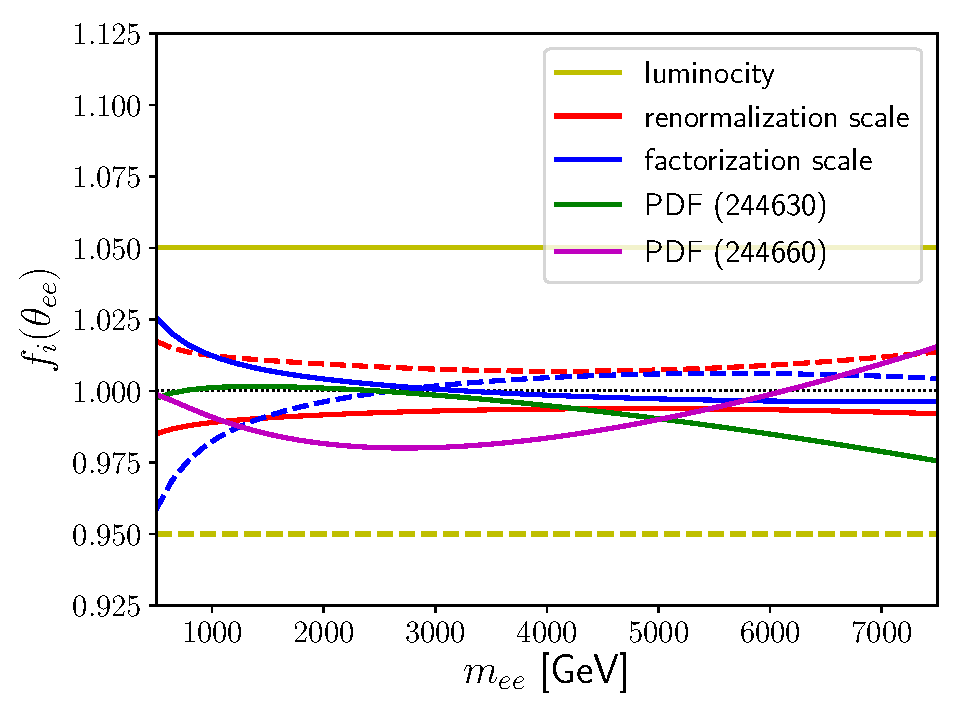
\includegraphics[width=0.5\hsize]{systematic.pdf}
  \caption{
    Form of the fitting function $f_{\mathrm{sys},i} (\bm{\theta}_f)$ evaluated with using the best fit values of $\bm{\theta}_f$ for several sources of systematic errors and $f=ee$.
    The yellow solid (dashed) line shows the result with luminosity error $+5\%$ ($-5\%$).
    The red and blue lines correspond to the different choices of the renormalization and the factorization scales, respectively, and the solid (dashed) line shows the result with $2Q$ ($Q/2$).
    The green and purple lines show results with different sets of the PDF, whose \texttt{LHAPDF6} IDs are given by 244630 and 244660, respectively.
  }
  \label{fig:systematic}
\end{figure}

To see how these errors mimic the WIMP signal, we show the form of $f_{\mathrm{sys},i} (\bm{\theta}_f)$ in Fig.~\ref{fig:systematic} for the best fit values of $\bm{\theta}_f$ under the existence of several sources of errors with $f=ee$ as an example.
The yellow solid (dashed) line shows the result with luminosity error $+5\%$ ($-5\%$).
The red and blue lines correspond to the different choices of the renormalization and the factorization scales, respectively, and the solid (dashed) line shows the result with $2Q$ ($Q/2$).
The green and purple lines show results with different sets of the PDF.
The main event set is generated by the PDF set with \texttt{LHAPDF6} ID 244600 and the green (purple) line shows the result of the \texttt{LHAPDF6} ID 244630 (244660) as an example.
From the figure, we can see that there are various forms of $\mathcal{O}(1)\,\%$ smooth corrections, including some smooth dip-like structures, all of which are well-fitted by the fitting function $f_{\mathrm{sys},i}(\bm{\theta_f})$.
Accordingly, as we will see below around Fig.~\ref{fig:nlo2}, a part of the WIMP effect, in particular a smooth part away from its dip, is also well-fitted by this function, which may decrease the sensitivity of our method significantly.

Several comments on other possible sources of systematic errors are in order.
Considering effects of the error on the beam energy, we could not generate events at NLO due to the lack of sufficient computational power.
Instead, we checked at LO that the corresponding values of $\bm{\sigma}$ (assuming that the uncertainty of the beam energy is $1\,\%$) are small enough, and hence we simply ignored it.
Two of the remaining sources are the pile-up effect and the underlying event, but they may be thought of as negligible since we are focusing on the very clean signal of two energetic leptons.
Another one is the effect of higher order contributions to the cross section including the electroweak loop correction from SM particles and that of background processes that are not considered in our analysis.
It is in principle possible to estimate their effects through the simulation and improve the analysis but here we just leave it as a future task.
Related to this, we note here that a smooth change of the number of events in general, possibly including the uncertainty listed above, could be absorbed by a minimization procedure using some fitting function like in Eq.~\eqref{eq_f_theta}.
On the other hand, as we will discuss below, the WIMP signal can not be fully absorbed by the fit because of the sharp bend we mentioned before.

We have also neglected the systematic errors from the detector effect.
The main errors are expected to come from the lepton identification, in which some of the leptons in any process are overlooked or identified incorrectly, resulting in the mis-reconstruction of the event topology.
Again, it is expected that the small and smooth modification of the number of events may be absorbed into the choice of nuisance parameters, if the corresponding values of $\bm{\sigma}_f$ are properly taken into account in addition to the values in Tables
\ref{tab_sys_ee} and \ref{tab_sys_ev}.
What is dangerous is the possible jerky modification that mimics the WIMP signal, which may be induced by the detector setup, the complicated detector response to leptons, and so on.
Such unwanted fake signals may be avoided by checking the consistency between the electron and muon channels.
This is because there should be the same size signals at the same lepton invariant mass in both channels for the WIMP signal, while the detector response to electrons and muons is different and such a coincidence is not expected in general.
It may also be helpful to look for similar fake signals in different processes associated with several leptons.
The similar treatment may also be useful to reduce the fake signals from the so-called look-elsewhere effect.
In principle, systematic errors from the detector and the look-elsewhere effects should be evaluated by repeating pseudo experiments many times including the detector simulation, but it requires a huge computational power and the detailed information of the detector construction and setup.
Thus, in this section, we just assume that these errors are well controlled once the real experiment will start and focus on the theoretical uncertainties listed in tables.


%%%%%%%%%%%%%%%%%%%%%%%%%%%%%%%%%%%%%%%%%%%%%%%%%%
\subsubsection{Detection reach}
\label{sec_detection}
%%%%%%%%%%%%%%%%%%%%%%%%%%%%%%%%%%%%%%%%%%%%%%%%%%

\begin{figure}[t]
  \centering
  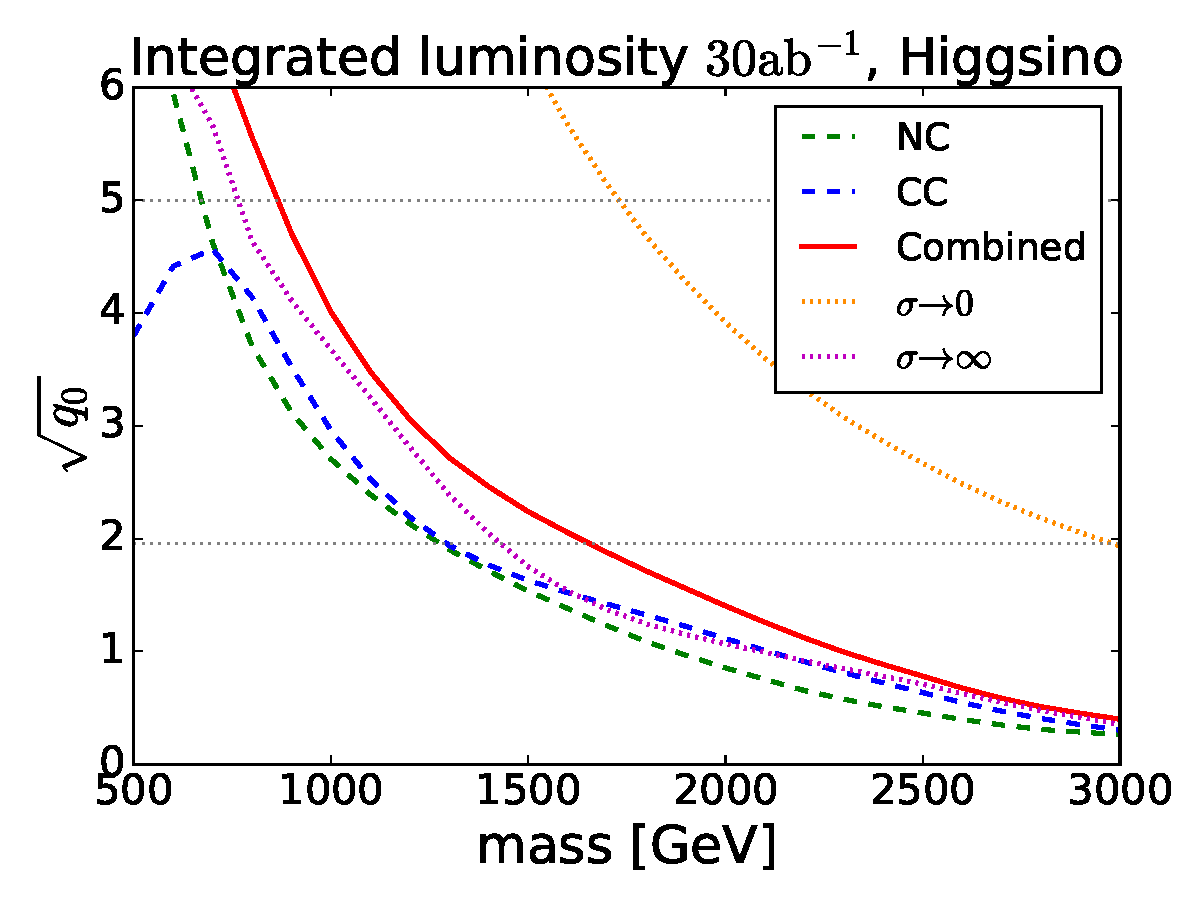
\includegraphics[width=0.48\hsize]{mchi_vs_sqq0_Higgsino.pdf}
  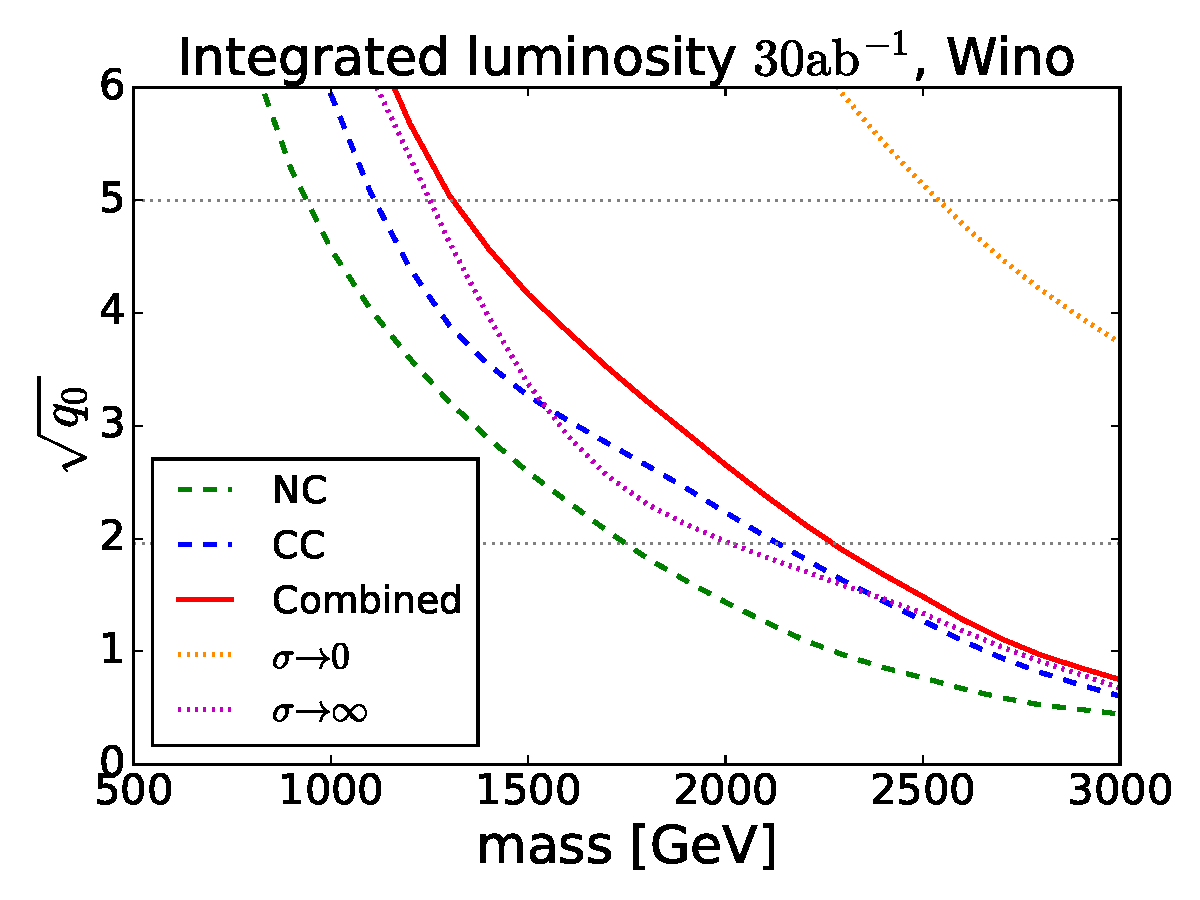
\includegraphics[width=0.48\hsize]{mchi_vs_sqq0_Wino.pdf}
  \caption{
    $\sqrt{q_0}$ as a function of the WIMP mass.
    \textbf{Left:} The figure for Higgsino.
    The green and blue dashed lines represent the results from the NC processes and the CC processes, respectively, while the red solid lines correspond to that from the combined analysis.
    The orange and purple lines denote the results from the combined analysis with the optimistic $\bm{\sigma}_f \to \bm{0}$ limit and those with conservative $\bm{\sigma}_f \to \infty$ limit, respectively.
    \textbf{Right:} The same for Wino.
  }
  \label{fig_mchi_vs_sqq0}
\end{figure}

\begin{figure}[t]
  \centering
  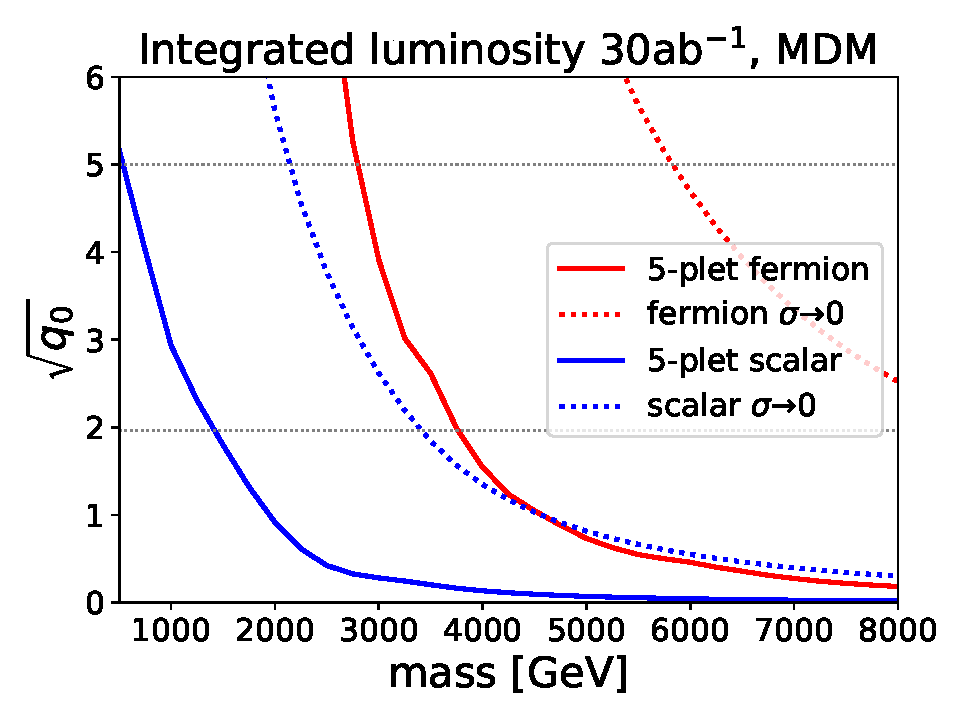
\includegraphics[width=0.48\hsize]{mchi_vs_sqq0_MDM.pdf}
  \caption{
    $\sqrt{q_0}$ as a function of the WIMP mass for the MDM models.
    The red and blue lines represent the results for 5-plet Majorana fermion and 5-plet real scalar, respectively, while the solid and dotted lines correspond to the result with and without the fitting procedure, respectively.
    All lines denote the combined results of the NC and CC processes.
  }
  \label{fig:mchi_vs_sqq0_MDM}
\end{figure}

Now we show the detection reach of WIMPs at future $100\,\mathrm{TeV}$ colliders.
In Fig.~\ref{fig_mchi_vs_sqq0}, we plot the value of $\sqrt{q_0}$ as a function of the WIMP mass, with the integrated luminosity $\mathcal{L}=30\,\mathrm{ab}^{-1}$.
As representative scenarios, we show the cases for Higgsino (the left figure) and Wino (the right figure).
In both figures, the green and blue dashed lines are the result obtained only from the NC processes and the CC processes, respectively.
We find that the CC processes are more sensitive to the effect of the WIMPs than the NC processes because of the larger cross section.
This result is consistent with Refs.~\cite{DiLuzio:2018jwd,Matsumoto:2018ioi}.
The sensitivity of the CC processes is weakened for $m \lesssim 700\, \mathrm{GeV}$ because of the lepton $p_T$ cut we have applied.\footnote
{
  We note here that the sensitivity of the CC processes depends on the lepton $p_T$ cut.
  For example, adopting the tighter cut, lepton-$p_T > 1\,\mathrm{TeV}$, the CC processes have almost no sensitivity to WIMPs with $m < 1\,\mathrm{TeV}$.
  Thus, particularly for the purpose of the Higgsino search, it is important to realize the lepton $p_T$ cut as low as $\sim 500\, \mathrm{GeV}$.
}
The combined results of the NC and CC processes are shown by the red solid lines.
By combining the two types of processes, the $5\sigma$ discovery reaches ($95\,\%$ C.L. bounds) for Higgsino and Wino are $850\,\mathrm{GeV}$ ($1.7\,\mathrm{TeV}$) and $1.3\,\mathrm{TeV}$ ($2.3\,\mathrm{TeV}$), respectively.
We find that the combination of the NC and CC processes improves the sensitivity of the WIMP mass.
Furthermore, if we understand all the systematic uncertainties quite well and effectively take the $\bm{\sigma}_f \to \bm{0}$ limit in the combined result, the detection reach will be pushed up significantly as shown by the orange dotted lines: $1.1\,\mathrm{TeV}$ Higgsino signal at well above $5\sigma$ level and a $4\sigma$ hint of the $2.9\,\mathrm{TeV}$ Wino.
These lines should be compared with the combined results and also with those obtained from the conservative analysis with $\bm{\sigma}_f \to \infty$ shown by the purple dotted lines, assuming no knowledge about sources of systematic errors.
The plot shows us that it is essential to reduce the systematic uncertainties for the detection of WIMPs through the NC and CC processes.

We also show the detection reach of the MDM scenario using both the NC and CC processes in Fig.~\ref{fig:mchi_vs_sqq0_MDM}.
The $5\sigma$ reaches are $2.8\,{\rm TeV}$ and $0.5\,{\rm TeV}$ for 5-plet fermion and 5-plet scalar, while the $95\,\%$ reaches are $3.8\,{\rm TeV}$ and $1.4\,{\rm TeV}$.
They will be improved up to $5.8\,{\rm TeV}$ and $2.2\,{\rm TeV}$ ($5\sigma$) and larger than $8\,{\rm TeV}$ and $3.4\,{\rm TeV}$ ($95\,\%$ C.L.) when the systematic errors are well understood.
If we assume the vanilla thermal freeze-out scenario, the mass should be around $10\,{\rm TeV}$ for both 5-plet fermion and scalar~\cite{Cirelli:2007xd}.
Thus, our method probes only a part of the allowed mass range for these multiplets.

\begin{figure}[t]
  \centering
  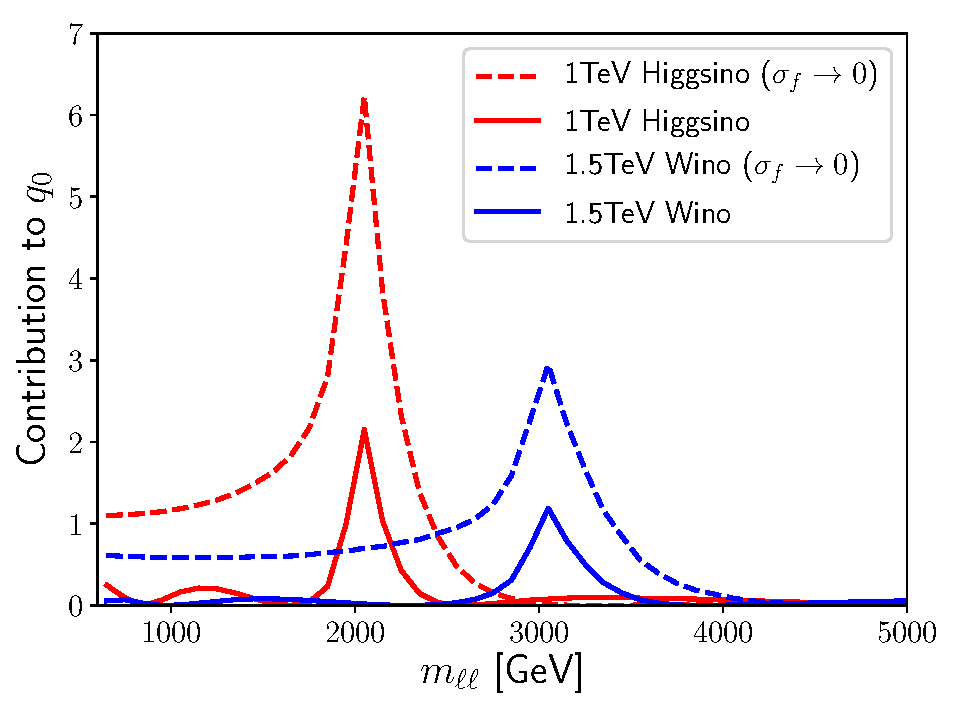
\includegraphics[width=0.495\hsize]{nlo2.pdf}
  \caption{
    Plot of the contribution of each bin to the value of $q_0$ for the NC processes.
    The red (blue) lines correspond to the $1\,\mathrm{TeV}$ Higgsino ($1.5\,\mathrm{TeV}$ Wino).
    The solid and dotted lines correspond to the results with the fitting procedure and those without it (\textit{i.e.,} the $\bm{\sigma}_f \to 0$ limit), respectively.
  }
  \label{fig:nlo2}
\end{figure}

Next, we plot in Fig.~\ref{fig:nlo2} the contribution of each bin to the value of $q_0$ to take a closer look at the significance of the dip structure, focusing on the NC processes as an example.
The red (blue) lines correspond to the $1\,\mathrm{TeV}$ Higgsino ($1.5\,\mathrm{TeV}$ Wino), while the solid and dotted lines correspond to the results with the fitting procedure and those without it (\textit{i.e.,} the $\bm{\sigma}_f \to 0$ limit), respectively.
We can see that most contributions come from the bins around the peak at $m_{\ell\ell} = 2m$.
This feature is clearer for the fitting based approach, where all the smooth parts of the correction are absorbed into the fit parameters, thus there is almost no contribution to $q_0$ from the bins other than $m_{\ell\ell} \sim 2m$.
Note also that, for the $\bm{\sigma}_f \to 0$ analysis, there are more contributions from the bins with lower $m_{\ell\ell}$ than those with higher $m_{\ell\ell}$, though sometimes the WIMP effect on the cross section is much larger in the latter bins.
This is just because of the difference in the number of events in each bin, that is $\mathcal{O}(10^7)$ for $500\,{\rm GeV} < m_{\ell\ell} < 600\,{\rm GeV}$, while $\mathcal{O}(10^3)$ for $4900\,{\rm GeV} < m_{\ell\ell} < 5000\,{\rm GeV}$ in our set up, for instance.
The similar behavior can be expected also for the CC processes.

So far, we have adopted the assumption that the distribution of the nuisance parameters is the Gaussian form and that the fitting function Eq.~\eqref{eq_f_theta} is sufficient for treating systematic errors.
In order to discuss the dependence of the results on these assumptions, we have repeated the same analysis using another distribution or fitting function.
In the former case, we have adopted the top-hat distribution: the likelihood function for the nuisance parameters $L'$ is given by
\begin{align}
  L' (\bm{\theta}_f ; \bm{\sigma}_f) \equiv \prod_\alpha
  \Theta \left( \sqrt{3}\ \sigma_{f,\alpha}
  - \left| \theta_{f,\alpha} \right| \right),
\end{align}
where $\Theta$ is the Heaviside step function.
This corresponds to the top-hat distribution of $\theta_{f,\alpha}$ with the variance $\sigma_{f,\alpha}^2$ for each $\alpha$.
As for an example of another fitting function, we have adopted a simple one-parameter extension of Eq.~\eqref{eq_f_theta}
\begin{align}
 f_{\mathrm{sys}, i} (\bm{\theta}_f) =
 e^{\theta_{f,1}} (1 - p_i)^{\theta_{f,2}}
 p_i^{(\theta_{f,3} + \theta_{f,4} \ln p_i + \theta_{f,5} \ln^2 p_i
 + \theta_{f,6} \ln^3 p_i)},\label{eq_6_param}
\end{align}
which consists of six parameters.
The variances of the nuisance parameters are estimated in the same way as Sec.~\ref{sec_statistical}, but now with the six parameters.

\begin{figure}[t]
  \centering
  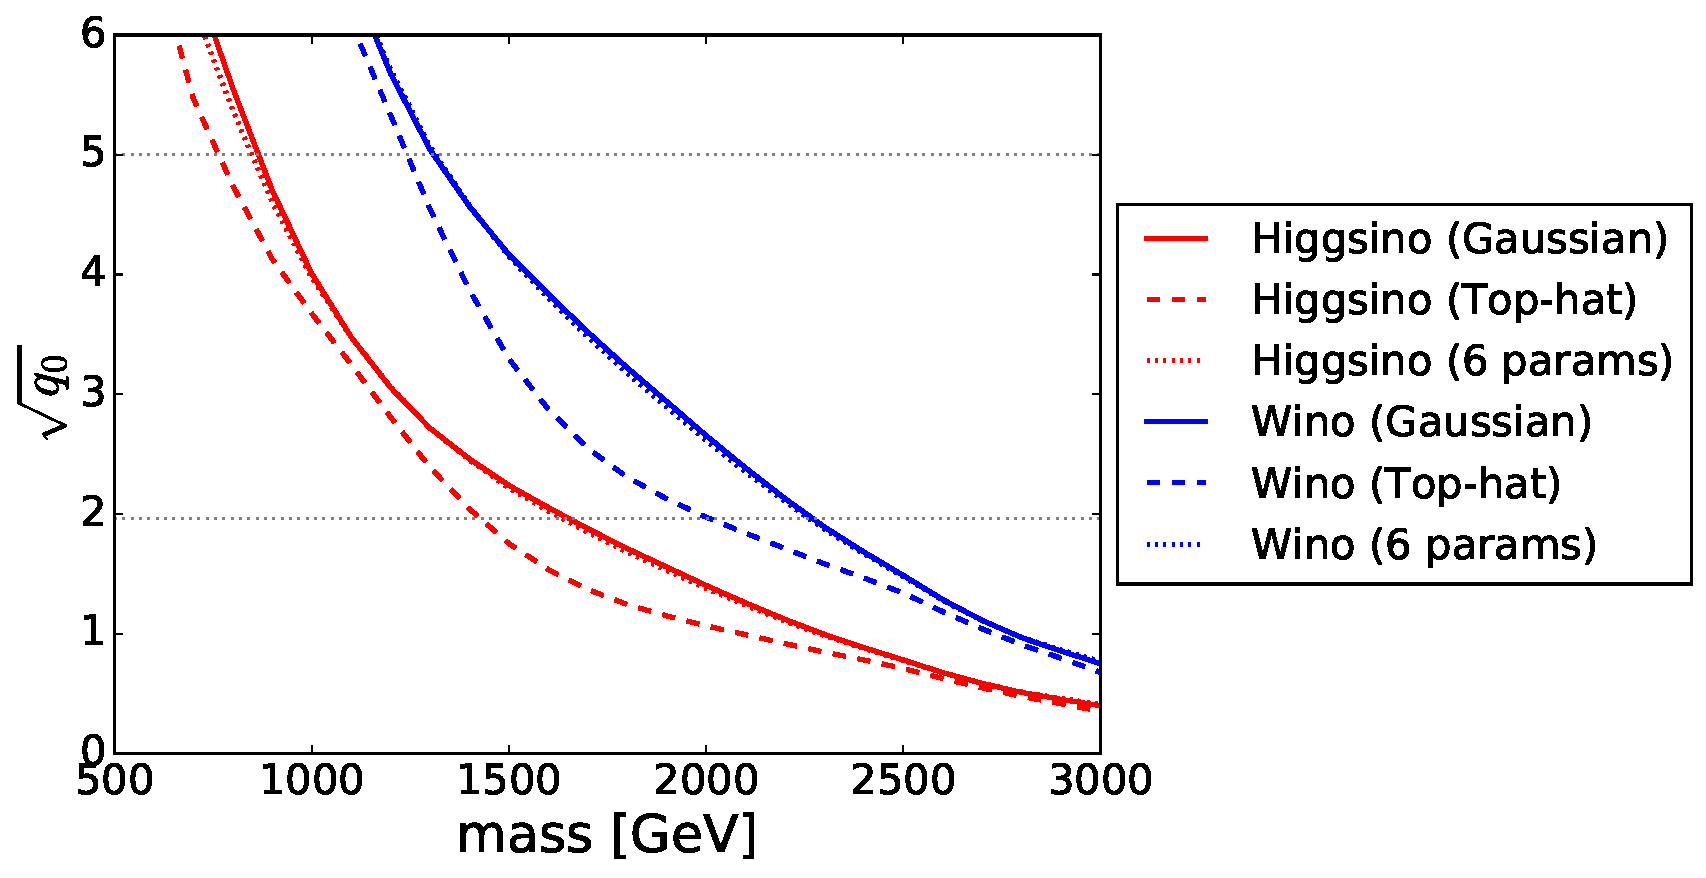
\includegraphics[width=0.7\linewidth]{mchi_vs_sqq0_comp.pdf}
  \caption{
    $\sqrt{q_0}$ as a function of the WIMP mass using both the NC and CC processes.
    The convention for the line colors is the same as Fig.~\ref{fig_mchi_vs_sqq0}.  The line styles denote the result same as Fig.~\ref{fig_mchi_vs_sqq0} (solid), that with the top-hat distribution (dashed), and that with the six parameters fitting function (dotted).
  }
  \label{fig_mchi_vs_sqq0_comp}
\end{figure}

In Fig.~\ref{fig_mchi_vs_sqq0_comp}, we show the corresponding results for Higgsino and Wino as an example.
The convention for the line colors is the same as Fig.~\ref{fig_mchi_vs_sqq0}, while the line styles denote different procedures: the dashed and dotted lines correspond to the result with the top-hat distribution and that with the six parameters fitting function, respectively, while solid lines are the same as Fig.~\ref{fig_mchi_vs_sqq0}.
From the figure, we can see that the choice of the distribution may slightly affect the result, while the addition of a nuisance parameter as Eq.~\eqref{eq_6_param} causes almost no effect.
The size of the effect of the choice of the distribution for the current estimation of errors $\bm{\sigma}_f$ is about $100\,\mathrm{GeV}$ ($200\,\mathrm{GeV}$) for the $5\sigma$ ($95\,\%$ C.L.) bounds.
We expect that such uncertainties due to the procedure to include the systematic errors will be reduced once the data from the real experiment (hence better understanding of the systematic errors) will become available.


%%%%%%%%%%%%%%%%%%%%%%%%%%%%%%%%%%%%%%%%%%%%%%%%%%
\subsubsection{Determination of WIMP properties}
\label{sec_property}
%%%%%%%%%%%%%%%%%%%%%%%%%%%%%%%%%%%%%%%%%%%%%%%%%%

In this subsection, we show that it is possible to determine the properties of the WIMPs from the NC and CC processes, thanks to the fact that we can study the $m_{\ell\ell}$ and $m_T$ distribution in great detail for these processes.
Some information about the mass, charge, and spin of the WIMPs can be extracted because the corrections to these distributions from the WIMPs are completely determined by these WIMP properties.
Firstly, we can extract the WIMP mass from the position of the dip-like structure in the correction since it corresponds to roughly twice the WIMP mass as we have shown in Sec.~\ref{sec:WIMP}.
Secondly, the overall size of the correction gives us information about the $SU(2)_L$ and $U(1)_Y$ charges.
The CC processes depend only on the $SU(2)_L$ charge, while the NC processes depend both on the $SU(2)_L$ and $U(1)_Y$ charges.
Consequently, we can obtain information about the gauge charges of the WIMPs from the NC and CC processes.

We now demonstrate the mass and charge determination of fermionic WIMPs.
This is equivalent to the determination of the parameter set $(m, C_1, C_2)$.
We generate the data assuming the SM $+$ WIMP model ($\mu=1$) with some specific values of $m, n, Y$, and $\kappa$, with which we obtain $(m, C_1, C_2)$.
We fix $\mu = 1$ for our theoretical model as well, and hence the theoretical predictions of the number of events also depend on these three parameters, $\bm{x}_f = \bm{x}_f (m, C_1, C_2)$.
We define the likelihood function $L(\check{\bm{x}}_f ; \bm{\theta}_f, m, C_1, C_2)$ in the same form as Eqs.~\eqref{eq_xtilde} and~\eqref{eq_L} with the theoretical prediction $\bm{x}_f$ now understood as a function of $(m, C_1, C_2)$, not of $\mu$.\footnote
{
  As shown in Eqs.\ \eqref{eq_C1} and \eqref{eq_C2}, $C_1$ and $C_2$ are positive quantities (and $C_2$ is discrete).
  In the figures, however, we extend the $C_1$ and $C_2$ axes down to negative regions just for presentation purposes.
}
The test statistic is defined as
%%
\begin{align}
  q (m, C_1, C_2)
  \equiv -2 \sum_f \ln \frac
  {L(\check{\bm{x}}_f ; \doublehat{\bm{\theta}}_f, m, C_1, C_2)}
  {L(\check{\bm{x}}_f ; \hat{\bm{\theta}}_f, \hat{m}, \hat{C}_1, \hat{C}_2)},
  \label{eq_q0f}
\end{align}
%%
where the parameters $(\{\hat{\bm{\theta}}_f\}, \hat{m}, \hat{C}_1, \hat{C}_2)$ maximize $\prod_f L(\check{\bm{x}}_f ; \bm{\theta}_f, m, C_1, C_2)$, while $\doublehat{\bm{\theta}}_f$ maximize
$L(\check{\bm{x}}_f ; \bm{\theta}_f, m, C_1, C_2)$ for fixed values of $(m, C_1, C_2)$.
It follows the chi-squared distribution with three degrees of freedom in the limit of a large number of events~\cite{Tanabashi:2018oca}.
The test statistic defined in this way examines the compatibility of a given WIMP model (i.e. a parameter set $(m, C_1, C_2)$) with the observed signal.


\begin{figure}[t]
  \centering
  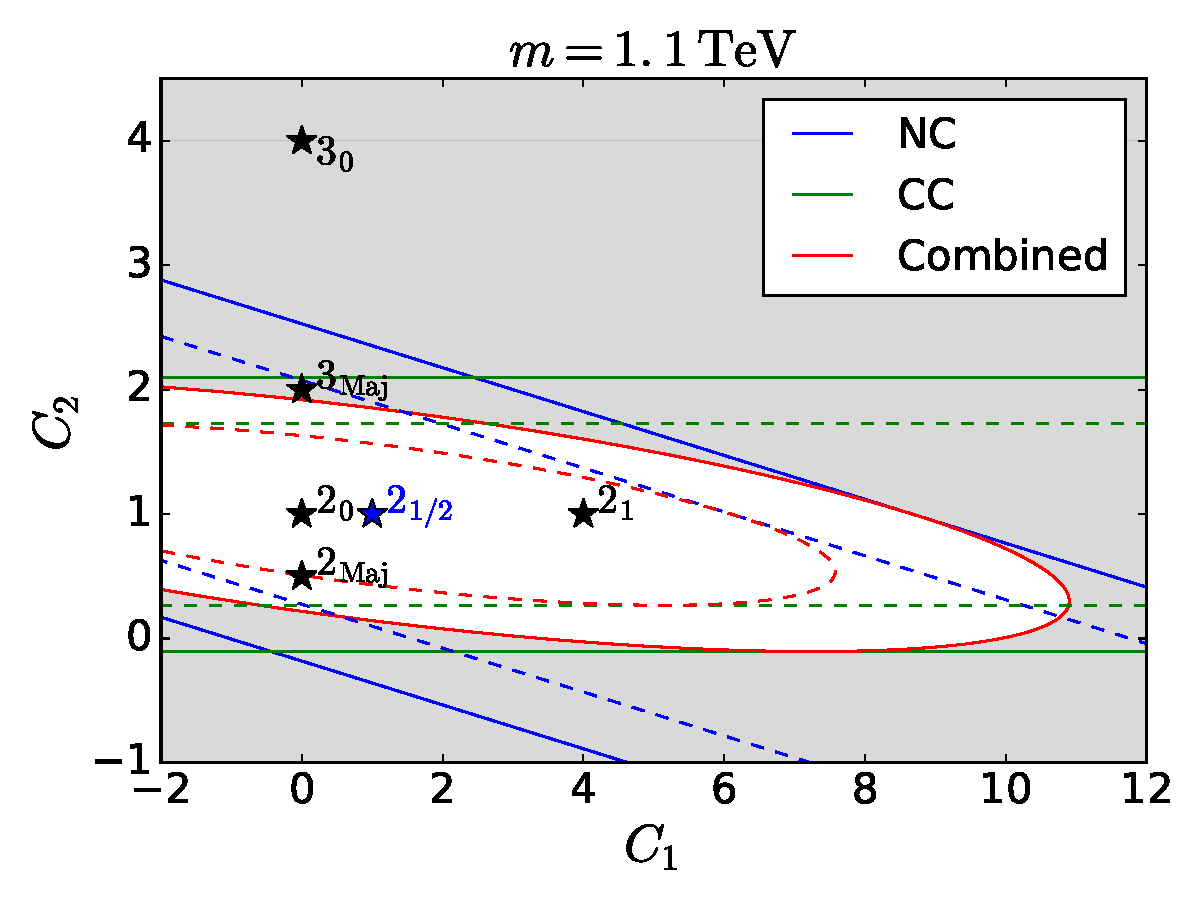
\includegraphics[width=0.5\linewidth]{C1_vs_C2_Higgsino.pdf}
  \caption{
    Contour of $\sqrt{q}$ in the $C_1~\mathrm{vs.}~C_2$ plane with $m = 1.1\,\mathrm{TeV}$, where we assume $1.1\,\mathrm{TeV}$ Higgsino signal.
    The dotted and solid lines denote $1\sigma$ and $2\sigma$ contours, respectively, and the gray region corresponds to the parameter space that is in tension with the observation at more than $2\sigma$ level.
    The blue, green, and red lines correspond to the result from the NC processes, the CC processes, and the combined analysis, respectively.
    Each star marker annotated as ``$n_Y$'' represents a point corresponding to a $SU(2)_L$ $n$-plet Dirac fermion with hypercharge $Y$, while that with ``$n_\mathrm{Maj}$'' corresponds to an $SU(2)_L$ $n$-plet Majorana fermion.
  }
  \label{fig_c1_c2}
\end{figure}

Once a deviation from the SM prediction is observed in a real experiment, we may determine $(m, C_1, C_2)$ using the above test statistic $q$.
In the following, we show the expected accuracy of the determination of $(m, C_1, C_2)$ for the case where there exists $1.1\,\mathrm{TeV}$ Higgsino.\footnote
{
  The expected significance is $3.5\sigma$ for $1.1\,\mathrm{TeV}$ Higgsino in our estimation.
  Even though it is slightly below the $5\sigma$ discovery, we take $1.1\,\mathrm{TeV}$ Higgsino as an example because it is a candidate of the thermal relic DM.
}

In Fig.~\ref{fig_c1_c2}, we show the contours of $1\sigma$ (dotted) and $2\sigma$ (solid) constraints, which correspond to the values $\sqrt{q}=1.9$ and $\sqrt{q}=2.8$, respectively, in the $C_1~\mathrm{vs.}~C_2$ plane for $m=1.1\,\mathrm{TeV}$.
The blue, green, and red lines denote the result obtained from the NC processes, the CC processes, and the combined analysis, respectively.
The models in the gray region are in more than $2\sigma$ tension with the observation.
We also show several star markers that correspond to the single $SU(2)_L$ multiplet contributions: the markers with ``$n_Y$'' represent an $SU(2)_L$ $n$-plet Dirac fermion with hypercharge $Y$, while those with ``$n_\mathrm{Maj}$'' an $SU(2)_L$ $n$-plet Majorana fermion.
Among them, the blue one with ``$2_{1/2}$'' corresponds to the Higgsino and to the best fit values in our analysis.
Both the NC and CC constraints are represented as straight bands in the $C_1~\mathrm{vs.}~C_2$ plane since each process depends on a specific linear combination of $C_1$ and $C_2$.
In particular, the CC constraint is independent of $C_1$, or $Y$.
In this sense, the NC and CC processes are complementary to each other, and thus we can separately constrain $C_1$ and $C_2$ only after combining these two results.
For instance, we can exclude a single fermionic $SU(2)_L$ multiplet with $n \neq 2$ at more than $2\sigma$ level, although each process by itself cannot exclude the possibility of $3_{\text{Maj}}$.
We can also constrain the hypercharge, yet it is not uniquely determined.
In addition to the Higgsino, the WIMP as an $SU(2)_L$ doublet Dirac fermion with $|Y|^2\lesssim 2$ or an $SU(2)_L$ doublet Majorana fermion with $|Y|^2\lesssim 5$ is still allowed.

\begin{figure}[t]
  \centering
  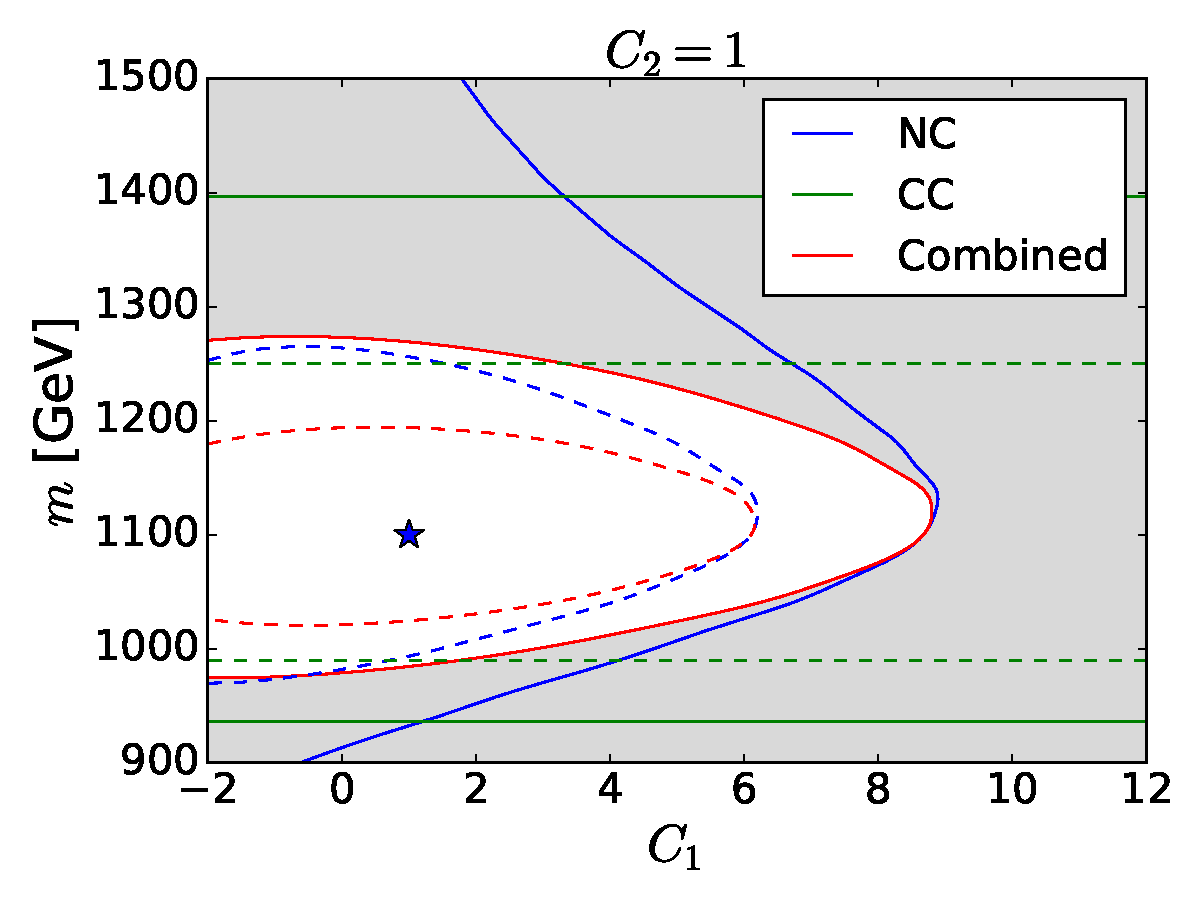
\includegraphics[width=0.48\linewidth]{C1_vs_mass_Higgsino.pdf}
  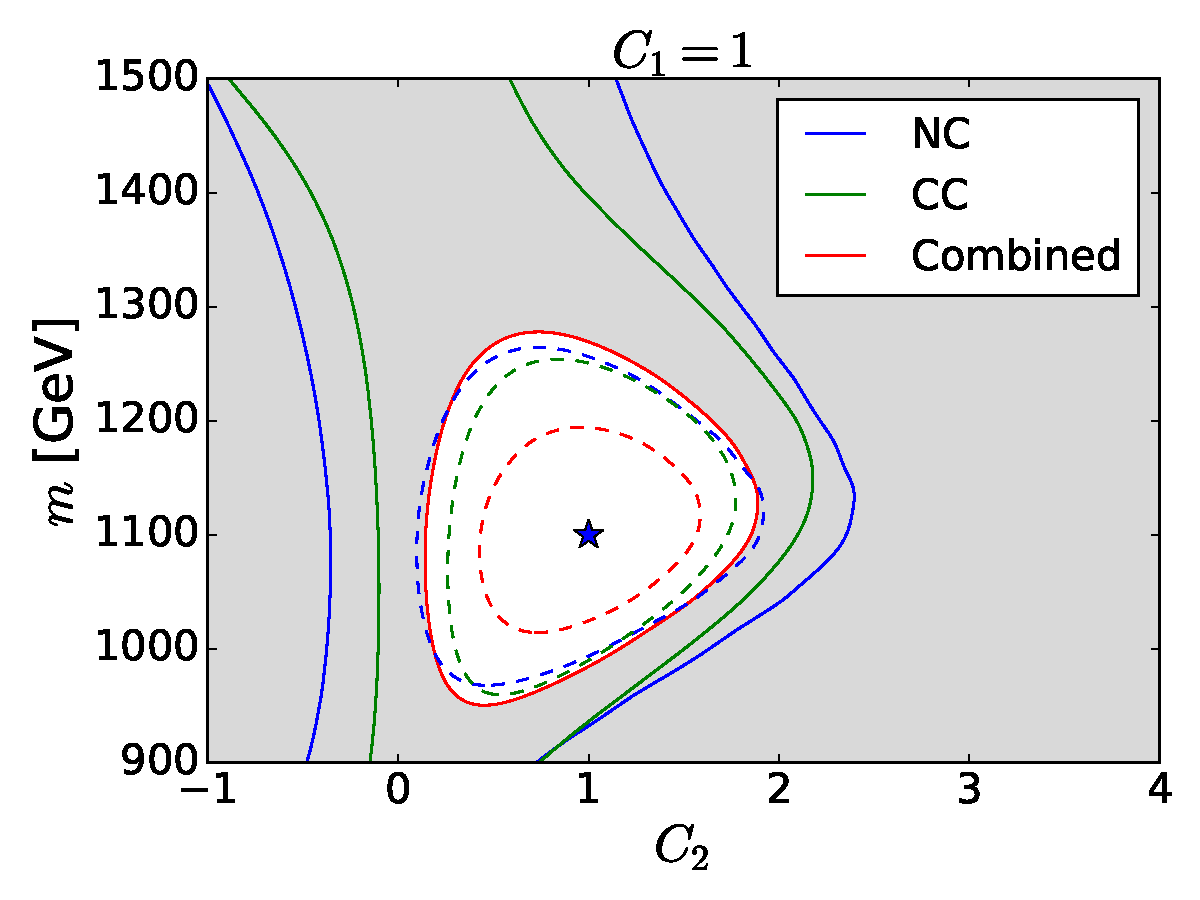
\includegraphics[width=0.48\linewidth]{C2_vs_mass_Higgsino.pdf}
  \caption{
    \textbf{Left:} Contour of $\sqrt{q}$ in the $C_1~\mathrm{vs.}~m$ plane with $C_2 = 1$, where we assume the $1.1\,\mathrm{TeV}$ Higgsino signal.
    The colors and styles of lines and the meaning of the gray region are the same as Fig.~\ref{fig_c1_c2}.
    The star maker corresponds to the true Higgsino property $(C_1, m) = (1, 1.1\,\mathrm{TeV})$.
    \textbf{Right:} Contour of $\sqrt{q}$ in the $C_2~\mathrm{vs.}~m$ plane for $C_1 = 1$, where we assume the $1.1\,\mathrm{TeV}$ Higgsino signal.
    The star maker corresponds to the true Higgsino property $(C_2, m) = (1, 1.1\,\mathrm{TeV})$.
 }
 \label{fig_c1_m}
\end{figure}

In Fig.~\ref{fig_c1_m}, we show the contour plots of $\sqrt{q}$ in the $C_1~\mathrm{vs.}~m$ plane with $C_2=1$ (left) and those in the $C_2~\mathrm{vs.}~m$ plane with $C_1=1$ (right).
The star marker in each panel shows the true values of parameters $(C_1, m) = (1, 1.1\,\mathrm{TeV})$ (left) and $(C_2, m) = (1, 1.1\,\mathrm{TeV})$ (right).
Again, by combining the NC and CC results, we can significantly improve the determination of WIMP properties, making $1\sigma$ and $2\sigma$ contours closed circles in the planes of our concern.
In particular, as red lines show, the combined analysis allows us to determine the observed WIMP mass at the level of $\mathcal{O}(10)\%$.

\begin{figure}[t]
  \centering
  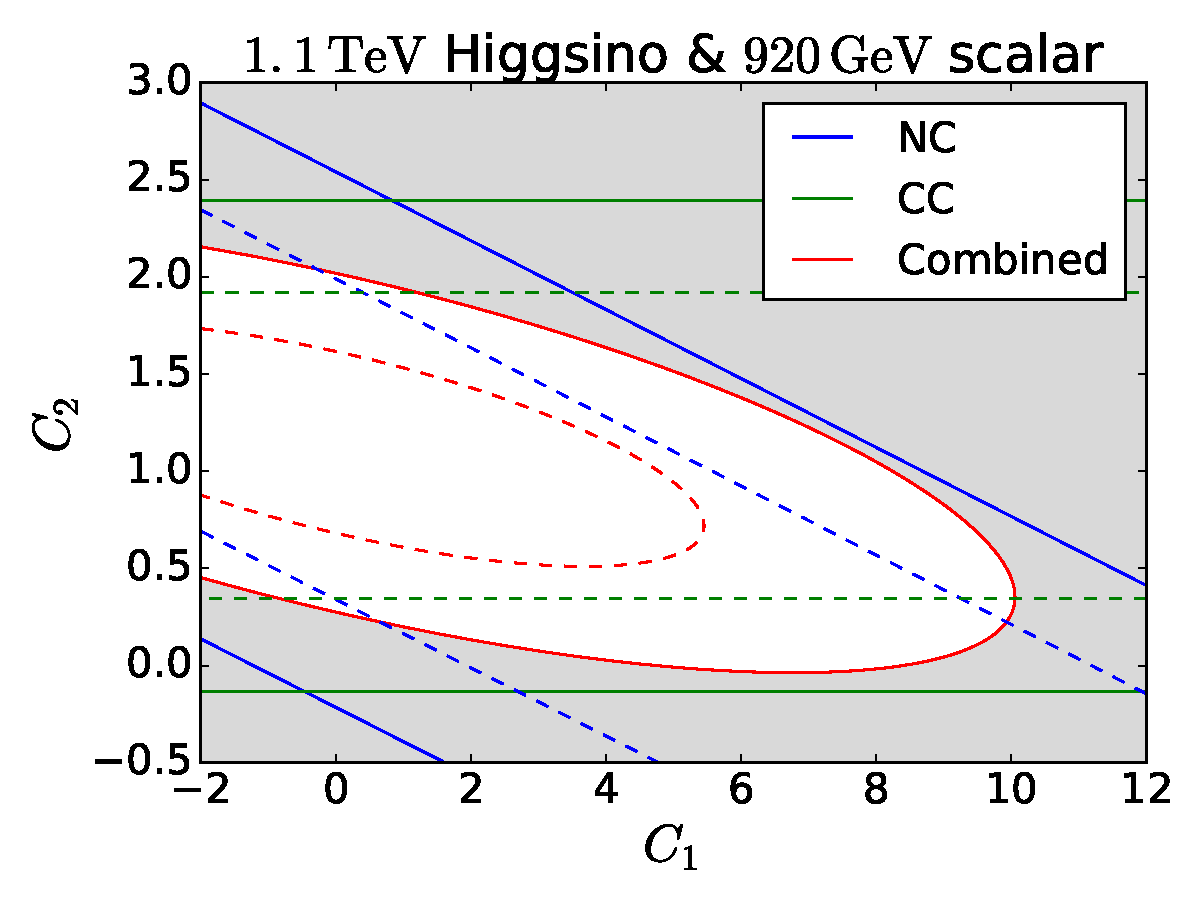
\includegraphics[width=0.5\linewidth]{C1_vs_C2_Higgsino_scalar.pdf}
  \caption{
    Contour of $\sqrt{q}$ in the $C_1~\mathrm{vs.}~C_2$ plane for the $1.1\,\mathrm{TeV}$ Higgsino signal, tested with the scalar WIMP assumption.
    The plane is defined as the scalar mass of $920\,\mathrm{GeV}$.
    The colors and styles of lines and the meaning of the gray region are the same as Fig.~\ref{fig_c1_c2}.
  }
  \label{fig_c1_c2_scalar}
\end{figure}

\begin{figure}[t]
  \centering
  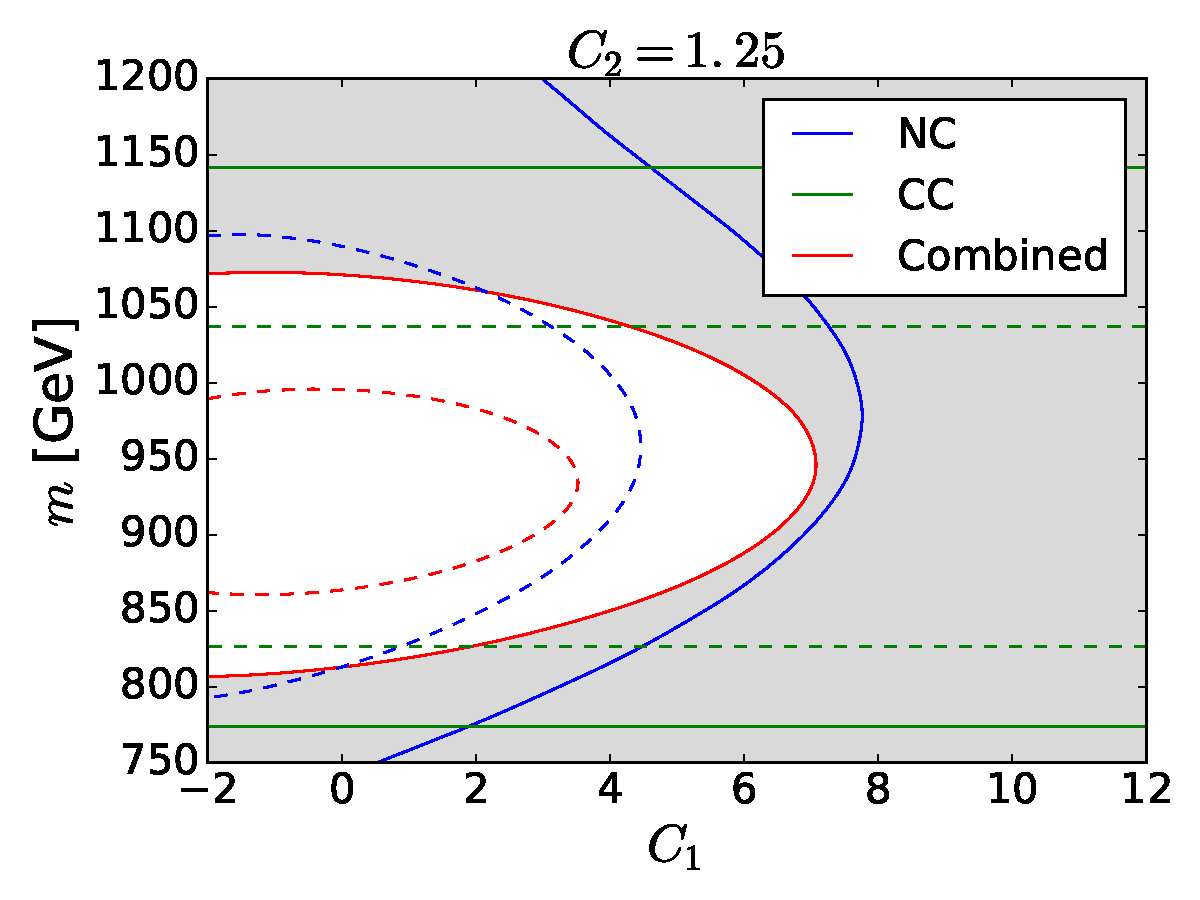
\includegraphics[width=0.48\linewidth]{C1_vs_mass_Higgsino_scalar.pdf}
  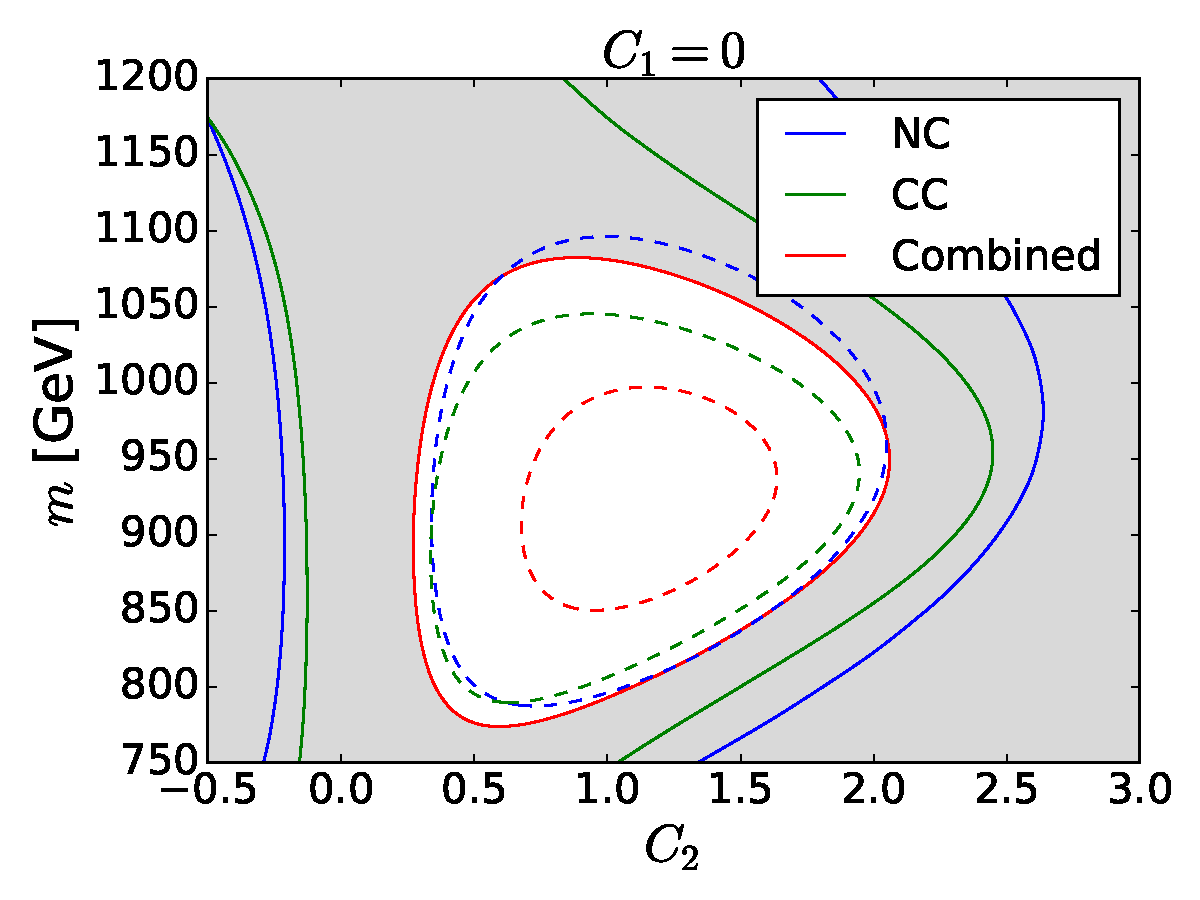
\includegraphics[width=0.48\linewidth]{C2_vs_mass_Higgsino_scalar.pdf}
  \caption{
    \textbf{Left:} Contour of $\sqrt{q}$ in the $C_1~\mathrm{vs.}~m$ plane with $C_2 = 1.25$ for the $1.1\,\mathrm{TeV}$ Higgsino signal, tested with the scalar WIMP assumption.
    The colors and styles of lines and the meaning of the gray region are the same as Fig.~\ref{fig_c1_c2}.
    \textbf{Right:} Contour  of $\sqrt{q}$ in the $C_2~\mathrm{vs.}~m$ plane with $C_1 = 0$ for the $1.1\,\mathrm{TeV}$ Higgsino signal, tested with the scalar WIMP assumption.
  }
  \label{fig_c1_m_scalar}
\end{figure}

Finally, we comment on the possibility of discriminating between fermionic and scalar WIMPs, whose difference comes from the loop function $f(x)$ (see Eq.~\eqref{eq_f}).
Here we repeat the same analysis explained above, assuming the $1.1\,\mathrm{TeV}$ Higgsino signal for example, but use the scalar loop function to evaluate the theoretical predictions $\bm{x}_f (m, C_1, C_2)$.
In Figs.~\ref{fig_c1_c2_scalar} and \ref{fig_c1_m_scalar}, we show the results in the $C_1$ vs. $C_2$ plane and the $C_1$ (or $C_2$) vs. $m$ plane, respectively, where one of the three parameters is fixed to its best fit value.
It is seen that, in the case of the $1.1\,\mathrm{TeV}$ Higgsino signal, it is hard to distinguish between the bosonic and fermionic WIMPs only with our method.
However, if a part of the WIMP properties (in particular its mass) is determined from another approach, our method may allow us to determine its spin correctly.

We also stress here that, with some favorable assumption about the observed signal, we may obtain some hint about its spin.
For example, if we assume that the observed signal composes a fraction of the dark matter in our Universe, the choice of the WIMP charges is significantly constrained.
Note from Fig.~\ref{fig_c1_c2_scalar} that the only choices of WIMP charges that allow the WIMP multiplet to contain an electrically neutral component are $(n,|Y|)=(3,0),(3,1),(4,1/2),(4,3/2)$, and $(5,0)_\text{real}$.
The last column of the table~\ref{tab:minimalDM-for-950scalar-section} shows proper choices of WIMP masses in order for their thermal relic abundances to become comparable with the dark matter abundance in the current Universe.
All of those values are somewhat larger than the central value of the mass of the observed signal, which means that the scalar interpretation of the signal cannot explain the whole of the dark matter relic abundance without introducing some non-thermal production mechanism.

\begin{table}[t]
  \centering
  \begin{tabular}{|c|ccc|}
    \hline
    $(n, Y)$           & $C_1$ & $C_2$ & $m_\text{DM}$[TeV] \\ \hline\hline
    $(3,0)_\text{real}$  &    0  &  0.25  & 2.5 \cite{Farina:2013mla}             \\
    $(3,          0)$  &    0  & 0.5   & 1.55 \cite{DelNobile:2015bqo}              \\
    $(3,          1)$  & 0.75  & 0.5   & 1.6 \cite{Farina:2013mla}               \\
    $(4,\frac{1}{2})$  & 0.25  & 1.25  & 2.4 \cite{Farina:2013mla}             \\
    $(4,\frac{3}{2})$  & 2.25  & 1.25  & 2.9 \cite{Farina:2013mla}             \\
    $(5,0)_\text{real}$  &    0  &  1.25  & 9.4 \cite{Farina:2013mla}          \\
    \hline
  \end{tabular}
  \caption{
    The scalar WIMPs that are compatible with the result in Fig.~\ref{fig_c1_c2_scalar}. The observed DM energy density is explained by the thermal relic of the WIMP with $m_{\text{DM}}$ shown in the fourth column.
  }
  \label{tab:minimalDM-for-950scalar-section}
\end{table}


%%%%%%%%%%%%%%%%%%%%%%%%%%%%%%%%%%%%%%%%%%%%%%%%%%
\subsection{Conclusion}
\label{seq:conclusion}
%%%%%%%%%%%%%%%%%%%%%%%%%%%%%%%%%%%%%%%%%%%%%%%%%%

In this section, we have discussed the indirect search of WIMPs at future $100\,\mathrm{TeV}$ hadron colliders based on the precision measurement of the production processes of a charged lepton pair and that of a charged lepton and a neutrino.
In particular, we have demonstrated that not only we can discover the WIMPs, but also we can determine their properties such as their masses, $SU(2)_L$ and $U(1)_Y$ charges, and  spins via the processes of our concern.
It is based on two facts: the high energy lepton production channel enables us to study its momentum distribution in great detail, and the WIMP correction shows characteristic features, including a dip-like structure as the final state invariant mass being twice the WIMP mass.
The latter feature also helps us to distinguish the WIMP signals from backgrounds and systematic errors, as they are not expected to show a dip-like structure.
In order to fully exploit the differences between the distributions of the WIMP signals and systematic errors, we have adopted the profile likelihood method as our statistical treatment.

First, we have shown in Fig.~\ref{fig_mchi_vs_sqq0} the detection reach of WIMPs from the NC processes (mediated by photon or $Z$-boson), the CC processes (mediated by $W$-boson), and the combination of these two results.
We have seen that the addition of the CC processes improves the detection reach from the previous analysis \cite{Chigusa:2018vxz}.
From the combined analysis, the bounds at the $5\sigma$ ($95\%$ C.L.) level for Higgsino and Wino are $850\,\mathrm{GeV}$ ($1.7\,\mathrm{TeV}$) and $1.3\,\mathrm{TeV}$ ($2.3\,\mathrm{TeV}$), respectively.
We have also shown the $5\sigma$ reach for 5-plet fermion and 5-plet scalar: $5.8\,{\rm TeV}$ and $2.2\,{\rm TeV}$ for the optimistic analysis and $2.8\,{\rm TeV}$ and $0.5\,{\rm TeV}$ for the analysis with a fitting procedure.
This result, particularly that for short lifetime Higgsino, indicates the importance of our method for the WIMP search.

Next, we have considered the determination of the mass and $SU(2)_L$ and $U(1)_Y$ charges of the observed WIMP.
By combining the NC and the CC events, the position and the height of the dip in the WIMP effect on the cross section gives us enough information for determining all the three parameters.
In Figs.~\ref{fig_c1_c2} and \ref{fig_c1_m}, we have shown the plots of the test statistics that test the validity of several choices of parameters.
As a result, the $SU(2)_L$ charge of the observed signal is correctly identified under the assumption of a single WIMP multiplet, and the $U(1)_Y$ charge and mass are also determined precisely.
In order for the determination of the WIMP spin, we have plotted the contours of the test statistics that test the validity of the scalar WIMP models with some fixed values of masses and charges.
The results are shown in Figs.~\ref{fig_c1_c2_scalar} and \ref{fig_c1_m_scalar}, which reveals that the spin is not completely determined by solely using our method.
Use of another approach to determine the WIMP properties, or of some assumption like that the observed signal corresponds to the dark matter in our Universe, may help us to obtain further information regarding the WIMP spin.

% \bibliographystyle{elsarticle-num}
% \bibliography{../phd}

\end{document}
